% =====================================================================
%  BÁO CÁO BÀI TẬP LỚN SỐ 2 - HỆ THỐNG QUẢN LÝ HỌC TẬP (LMS)
%  Biên dịch bằng XeLaTeX:
%      xelatex BaoCao_BTL2.tex
%      xelatex BaoCao_BTL2.tex      % chạy lần 2 để cập nhật mục lục
%
%  Ghi chú: preamble bám theo cấu hình yêu cầu. Nếu máy không có
%  Times New Roman, báo cáo tự chuyển sang DejaVu Serif để vẫn biên dịch.
% =====================================================================
\documentclass[a4paper,13pt]{extarticle}

% ==================================================
% 1. PAGE LAYOUT
% ==================================================
\usepackage[
    top=2cm,
    bottom=2cm,
    left=2.5cm,
    right=2.5cm
]{geometry}

\usepackage{setspace}
\setstretch{1.5}

\setlength{\parindent}{1.5em}
\setlength{\parskip}{3pt}
\usepackage{indentfirst}

% ==================================================
% 2. VIETNAMESE AND FONT CONFIGURATION
% Compile with XeLaTeX
% ==================================================
\usepackage{fontspec}
\usepackage{polyglossia}

\setdefaultlanguage{vietnamese}
\setotherlanguage{english}

\IfFontExistsTF{Times New Roman}{
    \setmainfont{Times New Roman}
}{
    \setmainfont{DejaVu Serif}
}
\IfFontExistsTF{Arial}{
    \setsansfont{Arial}
}{
    \setsansfont{DejaVu Sans}
}
\IfFontExistsTF{Courier New}{
    \setmonofont{Courier New}
}{
    \setmonofont{DejaVu Sans Mono}[Scale=0.85]
}

% ==================================================
% 3. MATHEMATICS
% ==================================================
\usepackage{amsmath}
\usepackage{amssymb}
\usepackage{systeme}

% ==================================================
% 4. GRAPHICS AND COLORS
% ==================================================
\usepackage{graphicx}
\usepackage{float}
\usepackage{caption}
\usepackage{tikz}
\usepackage{xcolor}
\usepackage{colortbl}

\definecolor{tableheader}{RGB}{220,230,241}
\definecolor{dkgreen}{RGB}{0,100,0}
\definecolor{gray}{RGB}{100,100,100}
\definecolor{mauve}{RGB}{128,0,128}
\definecolor{navy}{RGB}{20,55,120}

\captionsetup{font=small,labelfont=bf}
\usetikzlibrary{positioning,arrows.meta,shapes.geometric,fit,backgrounds,calc}

% ==================================================
% 5. TABLES
% ==================================================
\usepackage{array}
\usepackage{multirow}
\usepackage{multicol}
\usepackage{booktabs}
\usepackage{longtable}
\usepackage{tabularx}

\newcolumntype{L}[1]{>{\raggedright\arraybackslash}p{#1}}
\newcolumntype{C}[1]{>{\centering\arraybackslash}p{#1}}
\newcolumntype{Y}{>{\raggedright\arraybackslash}X}

\renewcommand{\arraystretch}{1.25}

% ==================================================
% 6. CODE LISTINGS
% ==================================================
\usepackage{listings}

\lstdefinestyle{sqlstyle}{
    language=SQL,
    basicstyle=\ttfamily\small,
    keywordstyle=\color{blue}\bfseries,
    commentstyle=\color{dkgreen}\itshape,
    stringstyle=\color{mauve},
    numbers=left,
    numberstyle=\tiny\color{gray},
    breaklines=true,
    frame=single,
    tabsize=4,
    showstringspaces=false,
    backgroundcolor=\color{white}
}

\lstdefinestyle{sqlappendix}{
    style=sqlstyle,
    basicstyle=\ttfamily\footnotesize,
    numbers=left,
    numberstyle=\tiny\color{gray}
}

% ==================================================
% 7. LIST CONFIGURATION
% ==================================================
\usepackage{enumitem}

\setlist[itemize]{
    leftmargin=2em,
    itemsep=3pt,
    topsep=3pt
}

\setlist[enumerate]{
    leftmargin=2em,
    itemsep=3pt,
    topsep=3pt
}

% ==================================================
% 8. HEADER AND FOOTER
% ==================================================
\usepackage{fancyhdr}
\usepackage{lastpage}

\pagestyle{fancy}
\fancyhf{}

\setlength{\headheight}{42pt}

\fancyhead[L]{
    \IfFileExists{figs/hcmut.png}{
        
\includegraphics[height=0.85cm]{figs/hcmut.png}
    }{}
}

\fancyhead[R]{
    \small
    \textbf{ĐẠI HỌC BÁCH KHOA}\\
    \textbf{ĐHQG TP. HỒ CHÍ MINH}
}

\fancyfoot[L]{\small BTL Hệ Cơ sở dữ liệu}
\fancyfoot[R]{\small Trang \thepage/\pageref*{LastPage}}

\renewcommand{\headrulewidth}{0.4pt}
\renewcommand{\footrulewidth}{0.4pt}

% ==================================================
% 9. SECTION FORMATTING
% ==================================================
\usepackage{titlesec}

\titleformat{\section}
    {\normalfont\Large\bfseries}
    {\thesection.}
    {0.5em}
    {}

\titleformat{\subsection}
    {\normalfont\large\bfseries}
    {\thesubsection}
    {0.5em}
    {}

\titleformat{\subsubsection}
    {\normalfont\normalsize\bfseries}
    {\thesubsubsection}
    {0.5em}
    {}

\titlespacing*{\section}{0pt}{18pt}{8pt}
\titlespacing*{\subsection}{0pt}{12pt}{5pt}

% ==================================================
% 10. TABLE OF CONTENTS
% ==================================================
\renewcommand{\contentsname}{MỤC LỤC}

% ==================================================
% 11. HYPERLINKS
% ==================================================
\usepackage[hidelinks]{hyperref}
\hypersetup{
    pdftitle={Báo cáo BTL2 - Hệ thống quản lý học tập (LMS)},
    pdfauthor={Nhóm BTL2 - CO3094},
    pdfsubject={Hệ Cơ sở dữ liệu}
}

% ==================================================
% 12. DOCUMENT INFORMATION
% ==================================================
\newcommand{\schoolName}{
    TRƯỜNG ĐẠI HỌC BÁCH KHOA\\
    ĐẠI HỌC QUỐC GIA TP. HỒ CHÍ MINH
}

\providecommand{\Tbl}[1]{\texttt{\detokenize{#1}}}
\newcommand{\code}[1]{\Tbl{#1}}

\begin{document}
\sloppy
\renewcommand{\contentsname}{MỤC LỤC}

% =====================================================================
% TITLE PAGE
% =====================================================================
\begin{titlepage}
\thispagestyle{empty}
\centering

{\Large\bfseries ĐẠI HỌC QUỐC GIA THÀNH PHỐ HỒ CHÍ MINH\\[2mm]}
{\Large\bfseries TRƯỜNG ĐẠI HỌC BÁCH KHOA\\[6mm]}


\includegraphics[width=2.8cm]{figs/hcmut.png}\\[8mm]

{\Large\bfseries BÁO CÁO BÀI TẬP LỚN SỐ 2}\\[3mm]
{\LARGE\bfseries HỆ THỐNG QUẢN LÝ HỌC TẬP (LMS)}\\[2mm]
{\large Phân tích, thiết kế, cài đặt và kiểm thử cơ sở dữ liệu}\\[10mm]

{\large Môn học: Hệ Cơ sở dữ liệu}\\[2mm]
{\large Mã môn học: CO3094}\\[10mm]

\begin{tabular}{p{5.2cm}p{7.4cm}}
\textbf{Nhóm thực hiện:} & Nhóm BTL2 \\[1mm]
\textbf{Thành viên:} &
\begin{tabular}[t]{@{}l@{}}
TV1: [Họ tên] -- [MSSV] \\
TV2: [Họ tên] -- [MSSV] \\
TV3: [Họ tên] -- [MSSV] \\
TV4: [Họ tên] -- [MSSV] \\
TV5: [Họ tên] -- [MSSV] \\
\end{tabular} \\[1mm]
\textbf{Giảng viên hướng dẫn:} & [Điền tên giảng viên] \\[1mm]
\textbf{Khoa:} & Khoa Khoa học và Kỹ thuật Máy tính \\
\end{tabular}

\vfill
{\large TP. Hồ Chí Minh, tháng 11 năm 2026}

\end{titlepage}

% =====================================================================
% FRONT MATTER
% =====================================================================
\pagenumbering{roman}
\tableofcontents
\clearpage
\listoftables
\clearpage
\listoffigures
\clearpage

\pagenumbering{arabic}

% =====================================================================
\section{Giới thiệu}
% =====================================================================

\subsection{Bối cảnh và mục tiêu}

Báo cáo này trình bày bài tập lớn số 2 của môn Hệ Cơ sở dữ liệu (CO3094), tiếp nối
bài tập lớn số 1 đã phân tích nghiệp vụ và thiết kế mô hình dữ liệu cho một hệ thống
quản lý học tập (Learning Management System -- LMS) theo mô hình của Trường Đại học
Bách khoa -- ĐHQG TP. Hồ Chí Minh. BTL1 đã chốt 20 thực thể, 2 quan hệ ISA và 28
mối quan hệ, kèm 17 quy tắc nghiệp vụ RB01--RB17. BTL2 yêu cầu hiện thực hóa mô hình
đó thành một cơ sở dữ liệu quan hệ chạy được, có dữ liệu mẫu, trigger, thủ tục, hàm,
và một ứng dụng thực sự gọi các đối tượng này.

Mục tiêu cụ thể:

\begin{itemize}
    \item Cài đặt đầy đủ 22 bảng quan hệ, khóa chính, khóa ngoại, ràng buộc miền giá trị
          và chỉ mục cần thiết.
    \item Sinh dữ liệu mẫu có ý nghĩa cho mọi bảng, tối thiểu 5 hàng mỗi bảng.
    \item Cài đặt 3 procedure CRUD trên bảng \Tbl{Enrollment}, 2 procedure truy vấn,
          2 function có cursor/IF/LOOP, và 13 trigger cho các quy tắc liên bảng.
    \item Xây dựng ứng dụng web Flask + giao diện SPA, phân quyền theo vai trò
          Student/Staff/Admin, gọi thật procedure/function từ màn hình.
    \item Kiểm thử tự động và kiểm thử đầu-cuối, ghi lại bằng chứng trung thực.
\end{itemize}

\subsection{Phạm vi và cách tiếp cận}

Phạm vi dữ liệu bám theo BTL1: tài khoản, khoa, sinh viên, giảng viên, quản trị viên,
học kỳ, môn học, thành phần môn học, lớp học phần, ghi danh, thông báo, tài nguyên,
đánh giá, bài tập, bài nộp, quiz, điểm và phản hồi. Ứng dụng chỉ phục vụ mục đích
minh họa học thuật, không phải hệ thống production.

Cách tiếp cận gồm bốn lớp: (1) tầng CSDL MySQL với schema, constraint, trigger,
procedure, function; (2) tầng truy cập dữ liệu Python dùng PyMySQL; (3) tầng dịch vụ
và API Flask; (4) tầng giao diện SPA offline dùng Bootstrap đã vendored. Mọi thao tác
ghi \Tbl{Enrollment} trên giao diện đều đi qua procedure, không dùng câu lệnh
\Tbl{INSERT}/\Tbl{UPDATE}/\Tbl{DELETE} trực tiếp.

\subsection{Kết quả đạt được}

\begin{table}[H]
\centering
\caption{Tóm tắt kết quả định lượng của bài tập}
\label{tab:summary}
\begin{tabular}{@{}L{8.2cm}C{4.8cm}@{}}
\toprule
\rowcolor{tableheader}
\textbf{Hạng mục} & \textbf{Kết quả} \\
\midrule
Bảng quan hệ & 22 bảng, 119 cột \\
Khóa ngoại / UNIQUE / CHECK & 35 FK, 10 UNIQUE, 39 CHECK \\
Chỉ mục hỗ trợ & 15 index \\
Trigger & 13 trigger \\
Stored procedure & 5 procedure \\
Stored function & 2 function \\
Dữ liệu mẫu & 22/22 bảng có $\geq 5$ hàng \\
Kiểm thử Python & 72 passed \\
Kiểm thử CSDL & \Tbl{DATABASE VERIFICATION: PASS} \\
Smoke API thật & 31/31 PASS \\
Kiểm thử trình duyệt & Chromium headless, không có lỗi console \\
\bottomrule
\end{tabular}
\end{table}

\subsection{Cấu trúc báo cáo}

Chương 2 mô tả quy trình thực hiện. Chương 3 trình bày thiết kế CSDL và kiểm kê
đầy đủ các bảng. Chương 4, 5, 6 lần lượt trình bày trigger, procedure và function.
Chương 7 mô tả ứng dụng, phân quyền và giao diện. Chương 8 tổng hợp kiểm thử.
Chương 9 là phân công, kết luận và hạn chế. Phần phụ lục chứa mã SQL tiêu biểu và
các lệnh kiểm tra.

% =====================================================================
\section{Quy trình thực hiện}
% =====================================================================

\subsection{Khảo sát và phân tích nghiệp vụ}

Nhóm kế thừa kết quả BTL1: mô hình ERD, 20 thực thể, 2 quan hệ ISA
(\Tbl{Student}/\Tbl{Staff}/\Tbl{Admin} là các \Tbl{UserAccount}), 28 mối quan hệ và
17 quy tắc RB01--RB17. Các quy tắc được phân loại theo nơi cài đặt:

\begin{itemize}
    \item \textbf{CHECK/UNIQUE/FK}: miền giá trị, duy nhất, tham chiếu.
    \item \textbf{Trigger}: quy tắc cần đọc nhiều hàng hoặc nhiều bảng, ví dụ trùng
          lịch, sĩ số, thuộc tính dẫn xuất \Tbl{Assignment.SubmissionCount}.
    \item \textbf{Procedure}: nghiệp vụ có nhiều bước và cần transaction, ví dụ thêm
          ghi danh phải kiểm tra tài khoản, lớp, sĩ số, trùng lặp.
    \item \textbf{Application/service}: phân quyền, ownership, kiểm tra dữ liệu đầu
          vào và các quy tắc trình bày.
\end{itemize}

\subsection{Thiết kế và chuẩn hóa}

Từ ERD, nhóm ánh xạ quan hệ 1:1, 1:N và N:M sang bảng. Các quan hệ ISA được cài đặt
bằng bảng cha \Tbl{UserAccount} và ba bảng con dùng chung khóa chính. Quan hệ N:M
\Tbl{CourseSection}--\Tbl{LearningResource} được cài đặt bằng bảng nối
\Tbl{Section_Resource}. Các thực thể yếu như \Tbl{SubmissionFile} dùng khóa chính
ghép. Thiết kế đạt dạng chuẩn 3 (3NF): mỗi bảng có khóa chính rõ ràng, thuộc tính
không khóa phụ thuộc đầy đủ vào khóa, không có phụ thuộc bắc cầu.

\subsection{Cài đặt và kiểm thử}

Thứ tự chạy CSDL được cố định: tạo database, tạo bảng, thêm khóa ngoại, thêm CHECK,
tạo index, tạo trigger, procedure, function, seed, rồi verify. Việc tách giai đoạn
giúp phát hiện lỗi tham chiếu sớm và cho phép chạy lại idempotent. Ứng dụng được cài
đặt song song với các test tầng repository để chứng minh API gọi đúng procedure.

\begin{figure}[H]
\centering
\begin{tikzpicture}[
    node distance=0.55cm and 0.65cm,
    box/.style={draw, rounded corners, fill=tableheader, minimum width=3.25cm,
                minimum height=1.05cm, align=center, font=\small},
    arrow/.style={-{Latex[length=2mm]}, thick}
]
\node[box] (s1) {1. Khảo sát\\nghiệp vụ BTL1};
\node[box, right=of s1] (s2) {2. Thiết kế\\ERD và chuẩn hóa};
\node[box, right=of s2] (s3) {3. Cài đặt\\schema + constraint};
\node[box, right=of s3] (s4) {4. Sinh\\dữ liệu mẫu};
\node[box, below=of s1] (s5) {5. Trigger, procedure,\\function};
\node[box, right=of s5] (s6) {6. Backend Flask\\và API};
\node[box, right=of s6] (s7) {7. Frontend SPA\\và phân quyền};
\node[box, right=of s7] (s8) {8. Kiểm thử, phản hồi\\và hoàn thiện};
\draw[arrow] (s1) -- (s2);
\draw[arrow] (s2) -- (s3);
\draw[arrow] (s3) -- (s4);
\draw[arrow] (s4.south) -- ++(0,-0.35) -| (s5.north);
\draw[arrow] (s5) -- (s6);
\draw[arrow] (s6) -- (s7);
\draw[arrow] (s7) -- (s8);
\end{tikzpicture}
\caption{Quy trình tám bước từ mô hình BTL1 đến ứng dụng và kiểm thử}
\label{fig:process}
\end{figure}

\subsection{Tiếp nhận phản hồi và sửa lỗi}

Sau khi có bản chạy đầu, nhóm rà lại theo rubric và phản hồi của người đánh giá.
Các lỗi thực tế đã sửa gồm: ánh xạ \Tbl{StudentCode} sai bảng, \Tbl{DayOfWeek} lệch
một đơn vị, thuộc tính HTML bị hỏng, thiếu tên tệp đính kèm, nút nộp bài vẫn hiện
khi hết lượt, tạo tài khoản Staff thiếu \Tbl{faculty_id}, và API quản trị chưa được
bảo vệ. Các thay đổi được ghi trong lịch sử Git với tiền tố \Tbl{feat}, \Tbl{fix},
\Tbl{test}, \Tbl{docs} và tham chiếu rubric.

% =====================================================================
\section{Thiết kế cơ sở dữ liệu}
% =====================================================================

\subsection{Mô hình tổng quan}

Hình~\ref{fig:erd-clusters} nhóm 22 bảng thành năm miền: định danh, học vụ, lớp học,
học liệu và đánh giá. Cách nhóm này phản ánh đường đi của dữ liệu trong ứng dụng:
một tài khoản thuộc một khoa; một sinh viên ghi danh vào lớp học phần; lớp có thông
báo, tài nguyên và đánh giá; đánh giá sinh ra bài tập/quiz, bài nộp, điểm và phản hồi.

\begin{figure}[H]
\centering
\begin{tikzpicture}[
    cluster/.style={draw, rounded corners, fill=tableheader, align=center,
                    font=\small, minimum width=4.2cm, minimum height=2.1cm},
    arrow/.style={-{Latex[length=2mm]}, thick},
    node distance=1.0cm and 1.2cm
]
\node[cluster] (id) {\textbf{Định danh}\\ \Tbl{UserAccount}, \Tbl{Student}\\ \Tbl{Staff}, \Tbl{Admin}, \Tbl{Faculty}};
\node[cluster, right=of id] (acad) {\textbf{Học vụ}\\ \Tbl{Semester}, \Tbl{Course}\\ \Tbl{CourseComponent}};
\node[cluster, right=of acad] (sec) {\textbf{Lớp học}\\ \Tbl{CourseSection}\\ \Tbl{Enrollment}};
\node[cluster, below=of id] (res) {\textbf{Học liệu}\\ \Tbl{Announcement}\\ \Tbl{LearningResource}, \Tbl{Section_Resource}};
\node[cluster, below=of acad] (assess) {\textbf{Đánh giá}\\ \Tbl{Assessment}, \Tbl{Assignment}\\ \Tbl{Quiz}, \Tbl{Grade}};
\node[cluster, below=of sec] (work) {\textbf{Bài nộp / phản hồi}\\ \Tbl{Submission}, \Tbl{SubmissionFile}\\ \Tbl{QuizAttempt}, \Tbl{Feedback}};
\draw[arrow] (id) -- node[above,font=\scriptsize]{1:N} (acad);
\draw[arrow] (acad) -- node[above,font=\scriptsize]{1:N} (sec);
\draw[arrow] (id) -- node[left,font=\scriptsize]{1:N} (res);
\draw[arrow] (sec) -- node[right,font=\scriptsize]{1:N} (res);
\draw[arrow] (sec) -- node[left,font=\scriptsize]{1:N} (assess);
\draw[arrow] (assess) -- node[above,font=\scriptsize]{1:N} (work);
\end{tikzpicture}
\caption{Nhóm bảng theo miền dữ liệu và quan hệ chính}
\label{fig:erd-clusters}
\end{figure}

\subsection{Kiểm kê 22 bảng, cột, khóa ngoại và CHECK}

Các bảng dưới đây được sinh trực tiếp từ \Tbl{database/schema/01_tables.sql},
\Tbl{database/constraints/02_foreign_keys.sql}, \Tbl{database/constraints/03_checks.sql},
\Tbl{database/indexes/04_indexes.sql} và \Tbl{docs/ROW_COUNTS.md}. Nhờ vậy, số cột,
khóa và biểu thức ràng buộc khớp với CSDL thật thay vì chép tay.

% =====================================================================
% AUTO-GENERATED from database/schema, constraints, indexes and ROW_COUNTS.md
% Do not edit by hand; the rows are generated from the SQL inventory files.
% =====================================================================
\providecommand{\Tbl}[1]{\texttt{\detokenize{#1}}}

{\footnotesize\setlength{\tabcolsep}{3pt}
\begin{longtable}{@{}C{0.6cm}L{3.0cm}C{1.2cm}L{2.9cm}C{0.9cm}C{0.9cm}C{0.9cm}L{4.1cm}@{}}
\caption{Danh mục 22 bảng của cơ sở dữ liệu}\label{tab:table-inventory}\\
\toprule
\rowcolor{tableheader}
\textbf{\#} & \textbf{Bảng} & \textbf{Cột} & \textbf{PK} & \textbf{FK} & \textbf{UQ} & \textbf{CK} & \textbf{Mục đích} \\
\midrule
\endfirsthead
\toprule
\rowcolor{tableheader}
\textbf{\#} & \textbf{Bảng} & \textbf{Cột} & \textbf{PK} & \textbf{FK} & \textbf{UQ} & \textbf{CK} & \textbf{Mục đích} \\
\midrule
\endhead
\bottomrule
\endfoot
1 & \Tbl{UserAccount} & 6 & \Tbl{UserID} & 0 & 1 & 3 & Tài khoản dùng chung; lưu email, họ tên, avatar, trạng thái, lần truy cập cuối. \\
2 & \Tbl{Faculty} & 3 & \Tbl{FacultyID} & 0 & 0 & 1 & Danh mục khoa. \\
3 & \Tbl{Student} & 3 & \Tbl{UserID} & 2 & 1 & 1 & Hồ sơ sinh viên (ISA của UserAccount) và khoa trực thuộc. \\
4 & \Tbl{Staff} & 2 & \Tbl{UserID} & 2 & 0 & 0 & Hồ sơ giảng viên/cán bộ (ISA của UserAccount) và khoa. \\
5 & \Tbl{Admin} & 1 & \Tbl{UserID} & 1 & 0 & 0 & Hồ sơ quản trị viên (ISA của UserAccount). \\
6 & \Tbl{Semester} & 5 & \Tbl{SemesterID} & 0 & 1 & 3 & Học kỳ theo năm học và số học kỳ. \\
7 & \Tbl{Course} & 6 & \Tbl{CourseID} & 2 & 1 & 2 & Môn học, số tín chỉ, khoa quản lý, người tạo. \\
8 & \Tbl{CourseComponent} & 4 & \Tbl{ComponentID} & 1 & 1 & 1 & Thành phần môn học: lý thuyết hoặc thực hành/bài tập. \\
9 & \Tbl{CourseSection} & 11 & \Tbl{SectionID} & 3 & 1 & 5 & Lớp học phần cụ thể trong học kỳ: lịch, phòng, sĩ số, giảng viên. \\
10 & \Tbl{Enrollment} & 5 & \Tbl{EnrollmentID} & 2 & 1 & 1 & Ghi danh sinh viên vào lớp học phần; bảng trung tâm của CRUD. \\
11 & \Tbl{Announcement} & 7 & \Tbl{AnnouncementID} & 2 & 0 & 1 & Thông báo của lớp học phần. \\
12 & \Tbl{LearningResource} & 7 & \Tbl{ResourceID} & 1 & 0 & 2 & Tài nguyên học tập dùng chung. \\
13 & \Tbl{Section_Resource} & 5 & \Tbl{SectionID, ResourceID} & 2 & 0 & 1 & Liên kết N:M giữa lớp học phần và tài nguyên. \\
14 & \Tbl{Assessment} & 8 & \Tbl{AssessmentID} & 2 & 0 & 2 & Đánh giá chung của lớp: assignment/quiz, điểm tối đa, số lần làm. \\
15 & \Tbl{Assignment} & 5 & \Tbl{AssessmentID} & 1 & 0 & 2 & Bài tập thuộc assessment; hạn nộp và số bài đã nộp (derived). \\
16 & \Tbl{AssignmentAttachment} & 2 & \Tbl{AssessmentID, AttachmentURL} & 1 & 0 & 1 & Tệp đính kèm của bài tập (metadata). \\
17 & \Tbl{Submission} & 9 & \Tbl{SubmissionID} & 3 & 1 & 4 & Bài nộp của sinh viên cho assignment. \\
18 & \Tbl{SubmissionFile} & 6 & \Tbl{SubmissionID, FileNo} & 1 & 0 & 2 & Tệp trong một bài nộp (metadata). \\
19 & \Tbl{Quiz} & 4 & \Tbl{AssessmentID} & 1 & 0 & 2 & Bài kiểm tra trắc nghiệm thuộc assessment. \\
20 & \Tbl{QuizAttempt} & 7 & \Tbl{AttemptID} & 2 & 1 & 3 & Một lần làm quiz của sinh viên. \\
21 & \Tbl{Grade} & 7 & \Tbl{GradeID} & 3 & 1 & 1 & Điểm của một enrollment cho một assessment. \\
22 & \Tbl{Feedback} & 6 & \Tbl{FeedbackID} & 3 & 0 & 1 & Nhận xét, có thể trả lời lồng nhau. \\
\end{longtable}}

{\footnotesize\setlength{\tabcolsep}{3pt}
\begin{longtable}{@{}L{3.2cm}L{12.4cm}@{}}
\caption{Danh sách cột của từng bảng (119 cột)}\label{tab:table-columns}\\
\toprule
\rowcolor{tableheader}
\textbf{Bảng} & \textbf{Các cột} \\
\midrule
\endfirsthead
\toprule
\rowcolor{tableheader}
\textbf{Bảng} & \textbf{Các cột} \\
\midrule
\endhead
\bottomrule
\endfoot
\Tbl{UserAccount} & \Tbl{UserID, Email, FullName, AvatarURL, AccountStatus, LastAccessAt} \\
\Tbl{Faculty} & \Tbl{FacultyID, FacultyName, FacultyNameEN} \\
\Tbl{Student} & \Tbl{UserID, StudentCode, FacultyID} \\
\Tbl{Staff} & \Tbl{UserID, FacultyID} \\
\Tbl{Admin} & \Tbl{UserID} \\
\Tbl{Semester} & \Tbl{SemesterID, AcademicYear, TermNo, StartDate, EndDate} \\
\Tbl{Course} & \Tbl{CourseID, CourseCode, CourseName, Credits, FacultyID, CreatedByAdminID} \\
\Tbl{CourseComponent} & \Tbl{ComponentID, CourseID, ComponentType, ComponentName} \\
\Tbl{CourseSection} & \Tbl{SectionID, ComponentID, SemesterID, PrimaryInstructorID, SectionCode, Capacity, SectionStatus, DayOfWeek, StartTime, EndTime, RoomCode} \\
\Tbl{Enrollment} & \Tbl{EnrollmentID, StudentID, SectionID, EnrollmentDate, EnrollmentStatus} \\
\Tbl{Announcement} & \Tbl{AnnouncementID, SectionID, PostedByStaffID, Title, Content, PostedAt, ExpiredAt} \\
\Tbl{LearningResource} & \Tbl{ResourceID, UploadedByStaffID, Title, Description, ResourceType, ResourceURL, UploadedAt} \\
\Tbl{Section_Resource} & \Tbl{SectionID, ResourceID, PostedAt, DisplayOrder, IsVisible} \\
\Tbl{Assessment} & \Tbl{AssessmentID, SectionID, CreatedByStaffID, Title, Description, CreatedAt, MaxScore, MaxAttempts} \\
\Tbl{Assignment} & \Tbl{AssessmentID, OpenDate, DueDate, AllowLateSubmission, SubmissionCount} \\
\Tbl{AssignmentAttachment} & \Tbl{AssessmentID, AttachmentURL} \\
\Tbl{Submission} & \Tbl{SubmissionID, AssignmentID, StudentID, GradedByStaffID, AttemptNo, SubmittedAt, SubmissionStatus, Score, GradedAt} \\
\Tbl{SubmissionFile} & \Tbl{SubmissionID, FileNo, FileName, FileURL, FileSize, UploadedAt} \\
\Tbl{Quiz} & \Tbl{AssessmentID, OpenTime, CloseTime, DurationMinutes} \\
\Tbl{QuizAttempt} & \Tbl{AttemptID, QuizID, StudentID, AttemptNo, StartedAt, FinishedAt, Score} \\
\Tbl{Grade} & \Tbl{GradeID, EnrollmentID, AssessmentID, GradedByStaffID, Score, GradedAt, IsPublished} \\
\Tbl{Feedback} & \Tbl{FeedbackID, SubmissionID, AuthorID, ParentFeedbackID, Content, CreatedAt} \\
\end{longtable}}

{\footnotesize\setlength{\tabcolsep}{2pt}
\begin{longtable}{@{}L{2.9cm}L{2.8cm}L{2.4cm}L{2.2cm}L{3.45cm}L{1.5cm}@{}}
\caption{35 khóa ngoại và quy tắc xóa/cập nhật}\label{tab:foreign-keys}\\
\toprule
\rowcolor{tableheader}
\textbf{Bảng con} & \textbf{Cột} & \textbf{Bảng cha} & \textbf{Cột cha} & \textbf{Constraint} & \textbf{ON DELETE} \\
\midrule
\endfirsthead
\toprule
\rowcolor{tableheader}
\textbf{Bảng con} & \textbf{Cột} & \textbf{Bảng cha} & \textbf{Cột cha} & \textbf{Constraint} & \textbf{ON DELETE} \\
\midrule
\endhead
\bottomrule
\endfoot
\Tbl{Student} & \Tbl{UserID} & \Tbl{UserAccount} & \Tbl{UserID} & \Tbl{fk_student_user} & \Tbl{CASCADE} \\
\Tbl{Student} & \Tbl{FacultyID} & \Tbl{Faculty} & \Tbl{FacultyID} & \Tbl{fk_student_faculty} & \Tbl{RESTRICT} \\
\Tbl{Staff} & \Tbl{UserID} & \Tbl{UserAccount} & \Tbl{UserID} & \Tbl{fk_staff_user} & \Tbl{CASCADE} \\
\Tbl{Staff} & \Tbl{FacultyID} & \Tbl{Faculty} & \Tbl{FacultyID} & \Tbl{fk_staff_faculty} & \Tbl{RESTRICT} \\
\Tbl{Admin} & \Tbl{UserID} & \Tbl{UserAccount} & \Tbl{UserID} & \Tbl{fk_admin_user} & \Tbl{CASCADE} \\
\Tbl{Course} & \Tbl{FacultyID} & \Tbl{Faculty} & \Tbl{FacultyID} & \Tbl{fk_course_faculty} & \Tbl{RESTRICT} \\
\Tbl{Course} & \Tbl{CreatedByAdminID} & \Tbl{Admin} & \Tbl{UserID} & \Tbl{fk_course_admin} & \Tbl{RESTRICT} \\
\Tbl{CourseComponent} & \Tbl{CourseID} & \Tbl{Course} & \Tbl{CourseID} & \Tbl{fk_component_course} & \Tbl{CASCADE} \\
\Tbl{CourseSection} & \Tbl{ComponentID} & \Tbl{CourseComponent} & \Tbl{ComponentID} & \Tbl{fk_section_component} & \Tbl{RESTRICT} \\
\Tbl{CourseSection} & \Tbl{SemesterID} & \Tbl{Semester} & \Tbl{SemesterID} & \Tbl{fk_section_semester} & \Tbl{RESTRICT} \\
\Tbl{CourseSection} & \Tbl{PrimaryInstructorID} & \Tbl{Staff} & \Tbl{UserID} & \Tbl{fk_section_instructor} & \Tbl{SET NULL} \\
\Tbl{Enrollment} & \Tbl{StudentID} & \Tbl{Student} & \Tbl{UserID} & \Tbl{fk_enrollment_student} & \Tbl{RESTRICT} \\
\Tbl{Enrollment} & \Tbl{SectionID} & \Tbl{CourseSection} & \Tbl{SectionID} & \Tbl{fk_enrollment_section} & \Tbl{RESTRICT} \\
\Tbl{Announcement} & \Tbl{SectionID} & \Tbl{CourseSection} & \Tbl{SectionID} & \Tbl{fk_announcement_section} & \Tbl{RESTRICT} \\
\Tbl{Announcement} & \Tbl{PostedByStaffID} & \Tbl{Staff} & \Tbl{UserID} & \Tbl{fk_announcement_staff} & \Tbl{RESTRICT} \\
\Tbl{LearningResource} & \Tbl{UploadedByStaffID} & \Tbl{Staff} & \Tbl{UserID} & \Tbl{fk_resource_staff} & \Tbl{RESTRICT} \\
\Tbl{Section_Resource} & \Tbl{SectionID} & \Tbl{CourseSection} & \Tbl{SectionID} & \Tbl{fk_sr_section} & \Tbl{CASCADE} \\
\Tbl{Section_Resource} & \Tbl{ResourceID} & \Tbl{LearningResource} & \Tbl{ResourceID} & \Tbl{fk_sr_resource} & \Tbl{CASCADE} \\
\Tbl{Assessment} & \Tbl{SectionID} & \Tbl{CourseSection} & \Tbl{SectionID} & \Tbl{fk_assessment_section} & \Tbl{RESTRICT} \\
\Tbl{Assessment} & \Tbl{CreatedByStaffID} & \Tbl{Staff} & \Tbl{UserID} & \Tbl{fk_assessment_staff} & \Tbl{RESTRICT} \\
\Tbl{Assignment} & \Tbl{AssessmentID} & \Tbl{Assessment} & \Tbl{AssessmentID} & \Tbl{fk_assignment_assessment} & \Tbl{CASCADE} \\
\Tbl{AssignmentAttachment} & \Tbl{AssessmentID} & \Tbl{Assignment} & \Tbl{AssessmentID} & \Tbl{fk_attachment_assignment} & \Tbl{CASCADE} \\
\Tbl{Submission} & \Tbl{AssignmentID} & \Tbl{Assignment} & \Tbl{AssessmentID} & \Tbl{fk_submission_assignment} & \Tbl{RESTRICT} \\
\Tbl{Submission} & \Tbl{StudentID} & \Tbl{Student} & \Tbl{UserID} & \Tbl{fk_submission_student} & \Tbl{RESTRICT} \\
\Tbl{Submission} & \Tbl{GradedByStaffID} & \Tbl{Staff} & \Tbl{UserID} & \Tbl{fk_submission_staff} & \Tbl{SET NULL} \\
\Tbl{SubmissionFile} & \Tbl{SubmissionID} & \Tbl{Submission} & \Tbl{SubmissionID} & \Tbl{fk_file_submission} & \Tbl{CASCADE} \\
\Tbl{Quiz} & \Tbl{AssessmentID} & \Tbl{Assessment} & \Tbl{AssessmentID} & \Tbl{fk_quiz_assessment} & \Tbl{CASCADE} \\
\Tbl{QuizAttempt} & \Tbl{QuizID} & \Tbl{Quiz} & \Tbl{AssessmentID} & \Tbl{fk_attempt_quiz} & \Tbl{RESTRICT} \\
\Tbl{QuizAttempt} & \Tbl{StudentID} & \Tbl{Student} & \Tbl{UserID} & \Tbl{fk_attempt_student} & \Tbl{RESTRICT} \\
\Tbl{Grade} & \Tbl{EnrollmentID} & \Tbl{Enrollment} & \Tbl{EnrollmentID} & \Tbl{fk_grade_enrollment} & \Tbl{RESTRICT} \\
\Tbl{Grade} & \Tbl{AssessmentID} & \Tbl{Assessment} & \Tbl{AssessmentID} & \Tbl{fk_grade_assessment} & \Tbl{RESTRICT} \\
\Tbl{Grade} & \Tbl{GradedByStaffID} & \Tbl{Staff} & \Tbl{UserID} & \Tbl{fk_grade_staff} & \Tbl{RESTRICT} \\
\Tbl{Feedback} & \Tbl{SubmissionID} & \Tbl{Submission} & \Tbl{SubmissionID} & \Tbl{fk_feedback_submission} & \Tbl{CASCADE} \\
\Tbl{Feedback} & \Tbl{AuthorID} & \Tbl{UserAccount} & \Tbl{UserID} & \Tbl{fk_feedback_author} & \Tbl{RESTRICT} \\
\Tbl{Feedback} & \Tbl{ParentFeedbackID} & \Tbl{Feedback} & \Tbl{FeedbackID} & \Tbl{fk_feedback_parent} & \Tbl{SET NULL} \\
\end{longtable}}

{\footnotesize\setlength{\tabcolsep}{3pt}
\begin{longtable}{@{}L{2.9cm}L{3.8cm}L{8.7cm}@{}}
\caption{39 ràng buộc CHECK theo miền giá trị và ngữ nghĩa}\label{tab:checks}\\
\toprule
\rowcolor{tableheader}
\textbf{Bảng} & \textbf{Constraint} & \textbf{Biểu thức} \\
\midrule
\endfirsthead
\toprule
\rowcolor{tableheader}
\textbf{Bảng} & \textbf{Constraint} & \textbf{Biểu thức} \\
\midrule
\endhead
\bottomrule
\endfoot
\Tbl{UserAccount} & \Tbl{ck_user_status} & \Tbl{`AccountStatus` IN ('ACTIVE', 'LOCKED', 'DISABLED')} \\
\Tbl{UserAccount} & \Tbl{ck_user_email} & \lstinline[basicstyle=\ttfamily\footnotesize]!`Email` LIKE '%_@_%._%' AND CHAR_LENGTH(`FullName`) > 0! \\
\Tbl{UserAccount} & \Tbl{ck_user_avatar} & \Tbl{CHAR_LENGTH(`AvatarURL`) > 0} \\
\Tbl{Faculty} & \Tbl{ck_faculty_name} & \Tbl{CHAR_LENGTH(`FacultyName`) > 0} \\
\Tbl{Student} & \Tbl{ck_student_code} & \Tbl{CHAR_LENGTH(`StudentCode`) BETWEEN 4 AND 20} \\
\Tbl{Semester} & \Tbl{ck_semester_term} & \Tbl{`TermNo` BETWEEN 1 AND 3} \\
\Tbl{Semester} & \Tbl{ck_semester_dates} & \Tbl{`StartDate` < `EndDate`} \\
\Tbl{Semester} & \Tbl{ck_semester_year} & \Tbl{`AcademicYear` REGEXP '^[0-9]{4}-[0-9]{4}$'} \\
\Tbl{Course} & \Tbl{ck_course_credits} & \Tbl{`Credits` BETWEEN 1 AND 10} \\
\Tbl{Course} & \Tbl{ck_course_code} & \Tbl{CHAR_LENGTH(`CourseCode`) > 0} \\
\Tbl{CourseComponent} & \Tbl{ck_component_type} & \Tbl{`ComponentType` IN ('THEORY', 'PRACTICE')} \\
\Tbl{CourseSection} & \Tbl{ck_section_capacity} & \Tbl{`Capacity` > 0} \\
\Tbl{CourseSection} & \Tbl{ck_section_status} & \Tbl{`SectionStatus` IN ('OPEN', 'CLOSED', 'CANCELLED')} \\
\Tbl{CourseSection} & \Tbl{ck_section_day} & \Tbl{`DayOfWeek` BETWEEN 1 AND 7} \\
\Tbl{CourseSection} & \Tbl{ck_section_time} & \Tbl{`StartTime` < `EndTime`} \\
\Tbl{CourseSection} & \Tbl{ck_section_room} & \Tbl{CHAR_LENGTH(`RoomCode`) > 0} \\
\Tbl{Enrollment} & \Tbl{ck_enrollment_status} & \Tbl{`EnrollmentStatus` IN ('ACTIVE', 'DROPPED', 'COMPLETED')} \\
\Tbl{Announcement} & \Tbl{ck_announcement_expiry} & \Tbl{`ExpiredAt` IS NULL OR `ExpiredAt` > `PostedAt`} \\
\Tbl{LearningResource} & \Tbl{ck_resource_type} & \Tbl{`ResourceType` IN ('DOCUMENT', 'SLIDE', 'VIDEO', 'LINK')} \\
\Tbl{LearningResource} & \Tbl{ck_resource_url} & \Tbl{CHAR_LENGTH(`ResourceURL`) > 0} \\
\Tbl{Section_Resource} & \Tbl{ck_sr_order} & \Tbl{`DisplayOrder` >= 0} \\
\Tbl{Assessment} & \Tbl{ck_assessment_score} & \Tbl{`MaxScore` > 0} \\
\Tbl{Assessment} & \Tbl{ck_assessment_attempts} & \Tbl{`MaxAttempts` IS NULL OR `MaxAttempts` > 0} \\
\Tbl{Assignment} & \Tbl{ck_assignment_period} & \Tbl{`OpenDate` < `DueDate`} \\
\Tbl{Assignment} & \Tbl{ck_assignment_count} & \Tbl{`SubmissionCount` >= 0} \\
\Tbl{AssignmentAttachment} & \Tbl{ck_attachment_url} & \Tbl{CHAR_LENGTH(`AttachmentURL`) > 0} \\
\Tbl{Submission} & \Tbl{ck_submission_attempt_no} & \Tbl{`AttemptNo` > 0} \\
\Tbl{Submission} & \Tbl{ck_submission_status} & \Tbl{`SubmissionStatus` IN ('DRAFT', 'SUBMITTED')} \\
\Tbl{Submission} & \Tbl{ck_submission_score} & \Tbl{`Score` IS NULL OR `Score` >= 0} \\
\Tbl{Submission} & \Tbl{ck_submission_grading} & \Tbl{(`Score` IS NULL AND `GradedAt` IS NULL) OR (`Score` IS NOT NULL AND `GradedAt` IS NOT NULL)} \\
\Tbl{SubmissionFile} & \Tbl{ck_file_no} & \Tbl{`FileNo` > 0} \\
\Tbl{SubmissionFile} & \Tbl{ck_file_size} & \Tbl{`FileSize` >= 0} \\
\Tbl{Quiz} & \Tbl{ck_quiz_time} & \Tbl{`OpenTime` < `CloseTime`} \\
\Tbl{Quiz} & \Tbl{ck_quiz_duration} & \Tbl{`DurationMinutes` > 0} \\
\Tbl{QuizAttempt} & \Tbl{ck_quiz_attempt_no} & \Tbl{`AttemptNo` > 0} \\
\Tbl{QuizAttempt} & \Tbl{ck_quiz_attempt_time} & \Tbl{`FinishedAt` IS NULL OR `FinishedAt` >= `StartedAt`} \\
\Tbl{QuizAttempt} & \Tbl{ck_quiz_attempt_score} & \Tbl{`Score` IS NULL OR `Score` >= 0} \\
\Tbl{Grade} & \Tbl{ck_grade_score} & \Tbl{`Score` >= 0} \\
\Tbl{Feedback} & \Tbl{ck_feedback_content} & \Tbl{CHAR_LENGTH(`Content`) > 0} \\
\end{longtable}}

{\footnotesize\setlength{\tabcolsep}{3pt}
\begin{longtable}{@{}L{4.8cm}L{3.0cm}L{7.6cm}@{}}
\caption{15 chỉ mục hỗ trợ lọc và join}\label{tab:indexes}\\
\toprule
\rowcolor{tableheader}
\textbf{Index} & \textbf{Bảng} & \textbf{Cột} \\
\midrule
\endfirsthead
\toprule
\rowcolor{tableheader}
\textbf{Index} & \textbf{Bảng} & \textbf{Cột} \\
\midrule
\endhead
\bottomrule
\endfoot
\Tbl{idx_user_account_status} & \Tbl{UserAccount} & \Tbl{`AccountStatus`} \\
\Tbl{idx_user_last_access} & \Tbl{UserAccount} & \Tbl{`LastAccessAt`} \\
\Tbl{idx_course_faculty} & \Tbl{Course} & \Tbl{`FacultyID`, `CourseCode`} \\
\Tbl{idx_component_course_type} & \Tbl{CourseComponent} & \Tbl{`CourseID`, `ComponentType`} \\
\Tbl{idx_section_schedule} & \Tbl{CourseSection} & \Tbl{`SemesterID`, `DayOfWeek`, `StartTime`, `EndTime`} \\
\Tbl{idx_section_instructor_semester} & \Tbl{CourseSection} & \Tbl{`PrimaryInstructorID`, `SemesterID`} \\
\Tbl{idx_enrollment_section_status} & \Tbl{Enrollment} & \Tbl{`SectionID`, `EnrollmentStatus`} \\
\Tbl{idx_enrollment_student_status} & \Tbl{Enrollment} & \Tbl{`StudentID`, `EnrollmentStatus`} \\
\Tbl{idx_announcement_section_posted} & \Tbl{Announcement} & \Tbl{`SectionID`, `PostedAt`} \\
\Tbl{idx_resource_staff_type} & \Tbl{LearningResource} & \Tbl{`UploadedByStaffID`, `ResourceType`} \\
\Tbl{idx_submission_assignment_status} & \Tbl{Submission} & \Tbl{`AssignmentID`, `SubmissionStatus`} \\
\Tbl{idx_submission_student_submitted} & \Tbl{Submission} & \Tbl{`StudentID`, `SubmittedAt`} \\
\Tbl{idx_quiz_attempt_student} & \Tbl{QuizAttempt} & \Tbl{`StudentID`, `StartedAt`} \\
\Tbl{idx_grade_assessment_published} & \Tbl{Grade} & \Tbl{`AssessmentID`, `IsPublished`} \\
\Tbl{idx_feedback_parent} & \Tbl{Feedback} & \Tbl{`ParentFeedbackID`} \\
\end{longtable}}

{\footnotesize\setlength{\tabcolsep}{3pt}
\begin{longtable}{@{}C{0.8cm}L{4.6cm}C{2.0cm}C{2.0cm}@{}}
\caption{Số hàng seed của 22 bảng (mọi bảng đạt $\geq 5$)}\label{tab:seed-counts}\\
\toprule
\rowcolor{tableheader}
\textbf{\#} & \textbf{Bảng} & \textbf{Số hàng} & \textbf{Đạt $\geq 5$?} \\
\midrule
\endfirsthead
\toprule
\rowcolor{tableheader}
\textbf{\#} & \textbf{Bảng} & \textbf{Số hàng} & \textbf{Đạt $\geq 5$?} \\
\midrule
\endhead
\bottomrule
\endfoot
1 & \Tbl{Admin} & 5 & Có \\
2 & \Tbl{Announcement} & 6 & Có \\
3 & \Tbl{Assessment} & 11 & Có \\
4 & \Tbl{Assignment} & 6 & Có \\
5 & \Tbl{AssignmentAttachment} & 6 & Có \\
6 & \Tbl{Course} & 5 & Có \\
7 & \Tbl{CourseComponent} & 8 & Có \\
8 & \Tbl{CourseSection} & 8 & Có \\
9 & \Tbl{Enrollment} & 16 & Có \\
10 & \Tbl{Faculty} & 5 & Có \\
11 & \Tbl{Feedback} & 7 & Có \\
12 & \Tbl{Grade} & 10 & Có \\
13 & \Tbl{LearningResource} & 8 & Có \\
14 & \Tbl{Quiz} & 5 & Có \\
15 & \Tbl{QuizAttempt} & 9 & Có \\
16 & \Tbl{Section_Resource} & 7 & Có \\
17 & \Tbl{Semester} & 5 & Có \\
18 & \Tbl{Staff} & 5 & Có \\
19 & \Tbl{Student} & 8 & Có \\
20 & \Tbl{Submission} & 13 & Có \\
21 & \Tbl{SubmissionFile} & 6 & Có \\
22 & \Tbl{UserAccount} & 18 & Có \\
\end{longtable}}


\subsection{Các quyết định thiết kế quan trọng}

\subsubsection{ISA dùng chung khóa chính}

\Tbl{Student}, \Tbl{Staff} và \Tbl{Admin} đều có khóa chính \Tbl{UserID} tham chiếu
\Tbl{UserAccount.UserID}. Cách này bảo đảm một tài khoản chỉ thuộc đúng một vai trò,
tránh trùng lặp email/họ tên, và cho phép xóa cascade hồ sơ khi xóa tài khoản.

\subsubsection{Bảng nối và thực thể yếu}

\Tbl{Section_Resource} là bảng nối N:M giữa lớp và tài nguyên, có khóa chính ghép
\Tbl{(SectionID, ResourceID)} và thuộc tính riêng \Tbl{DisplayOrder}.\\
\Tbl{AssignmentAttachment} và \Tbl{SubmissionFile} là thực thể yếu: khóa chính của
chúng chứa khóa của bảng cha, phù hợp với quan hệ 1:N.

\subsubsection{Thuộc tính dẫn xuất}

\Tbl{Assignment.SubmissionCount} là thuộc tính dẫn xuất được lưu thật và được trigger
cập nhật. Việc lưu giúp truy vấn thống kê nhanh, nhưng phải bảo đảm mọi thay đổi
\Tbl{Submission} đều kích hoạt tính lại. Đây là lý do có ba trigger
\Tbl{trg_submission_count_ai/ad/au}.

\subsubsection{Phân tách ràng buộc}

Ràng buộc miền giá trị dùng CHECK; ràng buộc duy nhất dùng UNIQUE; ràng buộc tham
chiếu dùng FK; ràng buộc liên bản ghi dùng trigger; ràng buộc quy trình dùng
procedure/service. Cách phân tách này tránh lạm dụng trigger và giữ schema dễ hiểu.

\subsection{Quy tắc nghiệp vụ và nơi cài đặt}

{\setlength{\tabcolsep}{3pt}\begin{longtable}{@{}L{1.1cm}L{7.0cm}L{4.1cm}L{2.3cm}@{}}
\caption{Ánh xạ 17 quy tắc nghiệp vụ sang cơ chế cài đặt}
\label{tab:rb}\\
\toprule
\rowcolor{tableheader}
\textbf{RB} & \textbf{Nội dung tóm tắt} & \textbf{Cơ chế chính} & \textbf{Trạng thái} \\
\midrule
\endfirsthead
\toprule
\rowcolor{tableheader}
\textbf{RB} & \textbf{Nội dung tóm tắt} & \textbf{Cơ chế chính} & \textbf{Trạng thái} \\
\midrule
\endhead
\bottomrule
\endfoot
RB01 & Tài khoản khóa/không hoạt động không được đăng nhập & Auth service kiểm tra \Tbl{AccountStatus} & Đã cài \\
RB02 & Mỗi lớp có tối đa một giảng viên phụ trách chính & Một cột \Tbl{PrimaryInstructorID} & Đã cài \\
RB03 & Không vượt sĩ số lớp & Trigger capacity + procedure & Đã cài \\
RB04 & Môn có lý thuyết + thực hành phải đăng ký nhóm hợp lệ & Ứng dụng/seed; chưa ép bằng trigger & Một phần \\
RB05 & Không trùng lịch giảng viên/phòng & Trigger schedule & Đã cài \\
RB06 & Mỗi môn có đúng một lý thuyết, tối đa một thực hành & UNIQUE + seed/ứng dụng & Một phần \\
RB07 & Chỉ Admin được khóa/mở tài khoản & \Tbl{require_role("ADMIN")} & Đã cài \\
RB08 & Chỉ Admin được tạo/sửa môn & \Tbl{require_role("ADMIN")} & Đã cài \\
RB09 & Chỉ sinh viên ACTIVE trong lớp mới được nộp/làm quiz & Trigger submission + service & Đã cài \\
RB10 & Bài nộp phải trong thời gian mở--hạn & Trigger submission & Đã cài \\
RB11 & Không vượt số lần làm/submit & UNIQUE + trigger + service & Đã cài \\
RB12 & Điểm nằm trong $[0, MaxScore]$ & Trigger grade + CHECK & Đã cài \\
RB13 & Chỉ giảng viên phụ trách được chấm & Staff service + trigger grade & Đã cài \\
RB14 & Quiz có thời gian mở/đóng và thời lượng hợp lệ & CHECK quiz & Đã cài \\
RB15 & Grade phải cùng section với assessment & Trigger grade & Đã cài \\
RB16 & Feedback phải thuộc submission, parent cùng submission & Trigger feedback & Đã cài \\
RB17 & Chỉ giảng viên phụ trách được tạo tài nguyên & Staff service & Đã cài \\
\end{longtable}}

Ghi chú trung thực: RB04 và RB06 được kiểm soát chủ yếu ở dữ liệu mẫu và tầng ứng
dụng, chưa có trigger ép buộc đầy đủ mọi tổ hợp đăng ký. Đây là giới hạn phạm vi của
bản demo, không phải tuyên bố đã hoàn thiện mọi quy tắc của LMS thật.

% =====================================================================
\section{Trigger}
% =====================================================================

\subsection{Vai trò và nguyên tắc}

Trigger được dùng cho bốn nhóm việc mà CHECK/UNIQUE/FK không làm được:

\begin{enumerate}
    \item \textbf{RB05 -- trùng lịch}: phải so sánh khoảng thời gian với nhiều hàng
          khác trong cùng học kỳ.
    \item \textbf{Thuộc tính dẫn xuất}: \Tbl{Assignment.SubmissionCount} phải được
          tính lại sau mọi thay đổi \Tbl{Submission}.
    \item \textbf{Sĩ số}: phải đếm số enrollment ACTIVE trước khi thêm/đổi lớp.
    \item \textbf{Kiểm tra liên bảng}: submission, grade và feedback cần JOIN nhiều
          bảng để xác định quyền và tính hợp lệ.
\end{enumerate}

\subsection{Danh sách 13 trigger}

{\footnotesize\setlength{\tabcolsep}{3pt}\begin{longtable}{@{}L{4.7cm}L{3.2cm}L{6.8cm}@{}}
\caption{13 trigger và phạm vi bảo vệ}
\label{tab:trigger-list}\\
\toprule
\rowcolor{tableheader}
\textbf{Trigger} & \textbf{Event / bảng} & \textbf{Mục đích} \\
\midrule
\endfirsthead
\toprule
\rowcolor{tableheader}
\textbf{Trigger} & \textbf{Event / bảng} & \textbf{Mục đích} \\
\midrule
\endhead
\bottomrule
\endfoot
\Tbl{trg_section_schedule_bi} & BEFORE INSERT \Tbl{CourseSection} & Chặn trùng lịch giảng viên/phòng khi thêm lớp \\
\Tbl{trg_section_schedule_bu} & BEFORE UPDATE \Tbl{CourseSection} & Chặn trùng lịch khi sửa, bỏ qua chính lớp đang sửa \\
\Tbl{trg_submission_count_ai} & AFTER INSERT \Tbl{Submission} & Tăng/tính lại \Tbl{SubmissionCount} \\
\Tbl{trg_submission_count_ad} & AFTER DELETE \Tbl{Submission} & Giảm/tính lại \Tbl{SubmissionCount} \\
\Tbl{trg_submission_count_au} & AFTER UPDATE \Tbl{Submission} & Tính lại assignment cũ và mới nếu đổi assignment \\
\Tbl{trg_enrollment_capacity_bi} & BEFORE INSERT \Tbl{Enrollment} & Chặn vượt sĩ số khi ghi danh \\
\Tbl{trg_enrollment_capacity_bu} & BEFORE UPDATE \Tbl{Enrollment} & Chặn vượt sĩ số khi đổi lớp/trạng thái \\
\Tbl{trg_submission_validate_bi} & BEFORE INSERT \Tbl{Submission} & Kiểm tra assignment, ghi danh ACTIVE, thời gian, số lần, điểm, giảng viên \\
\Tbl{trg_submission_validate_bu} & BEFORE UPDATE \Tbl{Submission} & Kiểm tra lại các quy tắc trên khi sửa \\
\Tbl{trg_grade_validate_bi} & BEFORE INSERT \Tbl{Grade} & Kiểm tra enrollment/assessment cùng section, điểm, giảng viên \\
\Tbl{trg_grade_validate_bu} & BEFORE UPDATE \Tbl{Grade} & Kiểm tra lại khi sửa điểm/assessment \\
\Tbl{trg_feedback_validate_bi} & BEFORE INSERT \Tbl{Feedback} & Feedback thuộc submission, parent cùng submission, người viết hợp lệ \\
\Tbl{trg_feedback_validate_bu} & BEFORE UPDATE \Tbl{Feedback} & Kiểm tra lại khi sửa feedback \\
\end{longtable}}

\subsection{Trigger trùng lịch RB05}

Điều kiện giao khoảng của hai lớp trong cùng \Tbl{SemesterID} và cùng
\Tbl{DayOfWeek} là:

\[
    \Tbl{NEW.StartTime} < \Tbl{cs.EndTime}
    \quad\land\quad
    \Tbl{cs.StartTime} < \Tbl{NEW.EndTime}.
\]

Trigger kiểm tra cả \Tbl{PrimaryInstructorID} và \Tbl{RoomCode}; khi UPDATE phải loại
trừ chính hàng đang sửa bằng \Tbl{cs.SectionID <> OLD.SectionID}. Test âm
\Tbl{04_trigger_expected_fail_schedule.sql} và
\Tbl{11_trigger_expected_fail_schedule_update.sql} chứng minh cả INSERT và UPDATE
đều bị chặn.

\subsection{Trigger thuộc tính dẫn xuất}

Công thức:

\[
    \Tbl{SubmissionCount} =
    \left|\{\,s \in \Tbl{Submission} \mid s.\Tbl{AssignmentID} = a.\Tbl{AssessmentID}\,\}\right|.
\]

Ba trigger AFTER INSERT/DELETE/UPDATE luôn đếm lại từ bảng thật, không cộng trừ mù.
Khi UPDATE đổi \Tbl{AssignmentID}, trigger tính lại cả assignment cũ và mới. Test
\Tbl{10_trigger_dml_matrix.sql} kiểm tra insert nhiều dòng, update đổi assignment,
update cột không khóa, delete và rollback.

\subsection{Ma trận DML}

\begin{table}[H]
\centering
\caption{Ma trận DML được bảo vệ bởi trigger}
\label{tab:trigger-dml}
\begin{tabular}{@{}L{4.4cm}L{3.1cm}L{6.0cm}@{}}
\toprule
\rowcolor{tableheader}
\textbf{Nhóm} & \textbf{Bảng} & \textbf{DML} \\
\midrule
Lịch học & \Tbl{CourseSection} & INSERT, UPDATE \\
Sĩ số & \Tbl{Enrollment} & INSERT, UPDATE \\
Bài nộp & \Tbl{Submission} & INSERT, UPDATE, DELETE \\
Điểm & \Tbl{Grade} & INSERT, UPDATE \\
Phản hồi & \Tbl{Feedback} & INSERT, UPDATE \\
\bottomrule
\end{tabular}
\end{table}

\subsection{Mã tiêu biểu}

\begin{lstlisting}[style=sqlstyle,caption={Trigger chặn trùng lịch khi INSERT (trích \Tbl{05_triggers.sql})},label={lst:schedule-trigger}]
CREATE TRIGGER `trg_section_schedule_bi`
BEFORE INSERT ON `CourseSection`
FOR EACH ROW
BEGIN
  IF EXISTS (
    SELECT 1
      FROM `CourseSection` cs
     WHERE cs.`SemesterID` = NEW.`SemesterID`
       AND cs.`DayOfWeek` = NEW.`DayOfWeek`
       AND NEW.`StartTime` < cs.`EndTime`
       AND cs.`StartTime` < NEW.`EndTime`
       AND (cs.`PrimaryInstructorID` = NEW.`PrimaryInstructorID`
            OR cs.`RoomCode` = NEW.`RoomCode`)
  ) THEN
    SIGNAL SQLSTATE '45000'
      SET MESSAGE_TEXT = 'Giang vien hoac phong bi trung lich trong hoc ky.';
  END IF;
END
\end{lstlisting}

% =====================================================================
\section{Stored procedure}
% =====================================================================

\subsection{Danh sách procedure}

{\footnotesize\setlength{\tabcolsep}{3pt}\begin{longtable}{@{}L{5.0cm}L{4.5cm}L{5.2cm}@{}}
\caption{5 stored procedure và mục đích}
\label{tab:procedures}\\
\toprule
\rowcolor{tableheader}
\textbf{Procedure} & \textbf{Tham số} & \textbf{Mục đích} \\
\midrule
\endfirsthead
\toprule
\rowcolor{tableheader}
\textbf{Procedure} & \textbf{Tham số} & \textbf{Mục đích} \\
\midrule
\endhead
\bottomrule
\endfoot
\Tbl{sp_InsertEnrollment} & \Tbl{student_id}, \Tbl{section_id}, \Tbl{status} & Thêm ghi danh có kiểm tra tài khoản, lớp, trùng, sĩ số, transaction \\
\Tbl{sp_UpdateEnrollment} & \Tbl{enrollment_id}, \Tbl{section_id}, \Tbl{status} & Sửa lớp/trạng thái; không đổi lớp/rút nếu đã có điểm \\
\Tbl{sp_DeleteEnrollment} & \Tbl{enrollment_id} & Xóa ghi danh nếu chưa có điểm \\
\Tbl{sp_GetStudentEnrollments} & \Tbl{student_id}, \Tbl{semester_id}, \Tbl{status}, \Tbl{limit}, \Tbl{offset} & Liệt kê ghi danh có JOIN, WHERE, ORDER BY, phân trang \\
\Tbl{sp_GetAssignmentStatistics} & \Tbl{section_id}, \Tbl{semester_id}, \Tbl{min_submissions} & Thống kê bài tập có aggregate, GROUP BY, HAVING \\
\end{longtable}}

\subsection{CRUD trên \texttt{Enrollment}}

Ba procedure CRUD thực hiện các kiểm tra sau:

\begin{itemize}
    \item \Tbl{sp_InsertEnrollment}: StudentID/SectionID dương; student tồn tại và
          tài khoản ACTIVE; section tồn tại; section OPEN; không trùng
          \Tbl{(StudentID, SectionID)}; nếu status ACTIVE thì đếm sĩ số so với
          \Tbl{Capacity}; khóa section bằng \Tbl{FOR UPDATE} để tránh đua.
    \item \Tbl{sp_UpdateEnrollment}: enrollment tồn tại; status hợp lệ; section mới
          tồn tại/OPEN; không trùng; kiểm tra sĩ số loại trừ chính enrollment đang sửa;
          không cho đổi lớp hoặc rút môn nếu đã có \Tbl{Grade}.
    \item \Tbl{sp_DeleteEnrollment}: enrollment tồn tại; từ chối xóa nếu có
          \Tbl{Grade}; xóa cứng khi chưa có điểm.
\end{itemize}

Cả ba dùng \Tbl{START TRANSACTION}, \Tbl{COMMIT} và handler
\Tbl{EXIT HANDLER FOR SQLEXCEPTION} để \Tbl{ROLLBACK} rồi \Tbl{RESIGNAL}. Nhờ đó lỗi
nghiệp vụ trả về mã \Tbl{45000} và được API ánh xạ thành HTTP 400 với mã
\Tbl{database_rule_violation}.

\subsection{Procedure truy vấn}

\begin{table}[H]
\centering
\caption{Đối chiếu yêu cầu của hai procedure truy vấn}
\label{tab:query-procedures}
\begin{tabular}{@{}L{4.0cm}L{5.0cm}L{5.0cm}@{}}
\toprule
\rowcolor{tableheader}
\textbf{Yêu cầu} & \Tbl{sp_GetStudentEnrollments} & \Tbl{sp_GetAssignmentStatistics} \\
\midrule
JOIN $\geq 2$ bảng & 7 bảng & 8 bảng \\
WHERE & student, semester, status & section, semester \\
ORDER BY & năm, học kỳ, mã môn, mã lớp & tỷ lệ hoàn thành, mã môn, mã lớp \\
Aggregate & Không & COUNT, MAX \\
GROUP BY / HAVING & Không & Có, theo ngưỡng bài nộp \\
Tham số UI & tab Ghi danh & tab Thống kê \\
\bottomrule
\end{tabular}
\end{table}

\subsection{Luồng UI -- API -- procedure}

\begin{figure}[H]
\centering
\begin{tikzpicture}[
    node distance=0.45cm,
    box/.style={draw, rounded corners, fill=tableheader, minimum width=5.4cm,
                minimum height=0.85cm, align=center, font=\small},
    arrow/.style={-{Latex[length=2mm]}, thick}
]
\node[box] (ui) {Giao diện Quản trị $\rightarrow$ Ghi danh};
\node[box, below=of ui] (api) {\Tbl{POST/PUT/DELETE /api/enrollments}};
\node[box, below=of api] (svc) {\Tbl{EnrollmentService}};
\node[box, below=of svc] (repo) {\Tbl{EnrollmentRepository}};
\node[box, below=of repo] (proc) {\Tbl{CALL sp_Insert/Update/DeleteEnrollment}};
\node[box, below=of proc] (db) {MySQL: trigger + FK + UNIQUE + CHECK};
\draw[arrow] (ui) -- (api);
\draw[arrow] (api) -- (svc);
\draw[arrow] (svc) -- (repo);
\draw[arrow] (repo) -- (proc);
\draw[arrow] (proc) -- (db);
\end{tikzpicture}
\caption{Đường đi của một thao tác CRUD Ghi danh}
\label{fig:crud-flow}
\end{figure}

\subsection{Mã tiêu biểu}

\begin{lstlisting}[style=sqlstyle,caption={Phần kiểm tra và transaction của \Tbl{sp_InsertEnrollment}},label={lst:insert-proc}]
START TRANSACTION;

SELECT COUNT(*) INTO v_exists
  FROM `Student` s
  JOIN `UserAccount` u ON u.`UserID` = s.`UserID`
 WHERE s.`UserID` = p_student_id
   AND u.`AccountStatus` = 'ACTIVE';

IF v_exists = 0 THEN
  SIGNAL SQLSTATE '45000'
    SET MESSAGE_TEXT = 'Sinh vien khong ton tai hoac tai khoan khong hoat dong.';
END IF;

SELECT `Capacity`, `SectionStatus`
  INTO v_capacity, v_section_status
  FROM `CourseSection`
 WHERE `SectionID` = p_section_id
 FOR UPDATE;

IF v_section_status <> 'OPEN' THEN
  SIGNAL SQLSTATE '45000'
    SET MESSAGE_TEXT = 'Lop hoc phan khong o trang thai OPEN.';
END IF;

INSERT INTO `Enrollment`
  (`StudentID`, `SectionID`, `EnrollmentDate`, `EnrollmentStatus`)
VALUES
  (p_student_id, p_section_id, CURRENT_TIMESTAMP, v_status);

SET v_new_id = LAST_INSERT_ID();
COMMIT;
\end{lstlisting}

% =====================================================================
\section{Stored function}
% =====================================================================

\subsection{Yêu cầu và cách đáp ứng}

Hai function đều \Tbl{READS SQL DATA}, không ghi dữ liệu, có cursor, handler
\Tbl{NOT FOUND}, vòng lặp \Tbl{LOOP}, \Tbl{IF}, validate đầu vào và truy vấn dữ liệu.

{\footnotesize\setlength{\tabcolsep}{3pt}\begin{longtable}{@{}L{4.6cm}L{10.2cm}@{}}
\caption{Đối chiếu yêu cầu rubric của hai function}
\label{tab:function-checklist}\\
\toprule
\rowcolor{tableheader}
\textbf{Yêu cầu} & \textbf{Bằng chứng} \\
\midrule
\endfirsthead
\toprule
\rowcolor{tableheader}
\textbf{Yêu cầu} & \textbf{Bằng chứng} \\
\midrule
\endhead
\bottomrule
\endfoot
Cursor & \Tbl{DECLARE cur_enrolled CURSOR FOR ...}; \Tbl{DECLARE cur_grades CURSOR FOR ...} \\
Handler & \Tbl{DECLARE CONTINUE HANDLER FOR NOT FOUND SET v_done = TRUE} \\
OPEN/FETCH/LOOP/CLOSE & Có đầy đủ trong cả hai function \\
IF/LOOP tính toán & Đếm submission; cộng điểm phần trăm đã publish \\
Query dữ liệu & JOIN \Tbl{Assignment}/\Tbl{Assessment}/\Tbl{Enrollment}/\Tbl{Submission}; JOIN \Tbl{Grade}/\Tbl{Assessment} \\
Validate input & ID NULL hoặc $\leq 0$ thì \Tbl{SIGNAL}; kiểm tra bản ghi tồn tại \\
Kết quả & \Tbl{DECIMAL(5,2)}, làm tròn 2 chữ số; trả 0.00 khi không có dữ liệu \\
\end{longtable}}

\subsection{\texttt{fn\_CalculateAssignmentCompletionRate}}

Công thức: số sinh viên ACTIVE đã có ít nhất một submission trạng thái
\Tbl{SUBMITTED} chia cho tổng số sinh viên ACTIVE của lớp, nhân 100. Nếu lớp không có
sinh viên ACTIVE, hàm trả \Tbl{0.00}. Hàm kiểm tra \Tbl{AssignmentID} dương và
assignment tồn tại trước khi mở cursor.

\subsection{\texttt{fn\_CalculateStudentAverageScore}}

Hàm duyệt các \Tbl{Grade} đã publish của một enrollment, quy đổi mỗi điểm theo
\Tbl{Score * 100 / MaxScore}, cộng dồn và chia cho số assessment đã publish. Đây là
chỉ số phân tích nội bộ, không phải công thức điểm chính thức của HCMUT. Nếu chưa có
grade published, hàm trả \Tbl{0.00}.

\subsection{Kết quả kiểm thử}

\begin{table}[H]
\centering
\caption{Kết quả gọi hàm trên dữ liệu mẫu}
\label{tab:function-results}
\begin{tabular}{@{}L{7.2cm}C{4.2cm}@{}}
\toprule
\rowcolor{tableheader}
\textbf{Biểu thức} & \textbf{Kết quả} \\
\midrule
\Tbl{fn_CalculateAssignmentCompletionRate(1)} & 100.00 \\
\Tbl{fn_CalculateAssignmentCompletionRate(6)} & 0.00 \\
\Tbl{fn_CalculateAssignmentCompletionRate(0)} & SIGNAL (expected fail) \\
\Tbl{fn_CalculateStudentAverageScore(1)} & 82.50 \\
\Tbl{fn_CalculateStudentAverageScore(8)} & 0.00 \\
\Tbl{fn_CalculateStudentAverageScore(-1)} & SIGNAL (expected fail) \\
\bottomrule
\end{tabular}
\end{table}

% =====================================================================
\section{Ứng dụng}
% =====================================================================

\subsection{Kiến trúc}

\begin{figure}[H]
\centering
\begin{tikzpicture}[
    node distance=0.45cm,
    box/.style={draw, rounded corners, fill=tableheader, minimum width=5.0cm,
                minimum height=0.8cm, align=center, font=\small},
    arrow/.style={-{Latex[length=2mm]}, thick}
]
\node[box] (browser) {Trình duyệt: SPA HTML/CSS/JS};
\node[box, below=of browser] (flask) {Flask Blueprint + validation};
\node[box, below=of flask] (service) {Service layer};
\node[box, below=of service] (repo) {Repository layer (PyMySQL)};
\node[box, below=of repo] (mysql) {MySQL 8.4: bảng, trigger, procedure, function};
\draw[arrow] (browser) -- node[right,font=\scriptsize]{HTTP/JSON} (flask);
\draw[arrow] (flask) -- (service);
\draw[arrow] (service) -- (repo);
\draw[arrow] (repo) -- node[right,font=\scriptsize]{SQL} (mysql);
\end{tikzpicture}
\caption{Kiến trúc bốn lớp của ứng dụng}
\label{fig:architecture}
\end{figure}

\subsection{Phân quyền theo vai trò}

Ứng dụng dùng mô hình demo \emph{chọn vai trò rồi chọn tài khoản}, không có mật khẩu.
Sau khi đăng nhập, Flask ghi \Tbl{user_id} và \Tbl{role} vào session. Mọi API được
bảo vệ bằng \Tbl{@require_role(...)}; thiếu session trả 401, sai vai trò trả 403.
Ngoài vai trò, service còn kiểm tra quyền sở hữu dữ liệu: Student chỉ thấy dữ liệu của
mình, Staff chỉ thấy lớp mình phụ trách, Admin không được chấm điểm (RB13).

\begin{table}[H]
\centering
\caption{Nhóm API và vai trò yêu cầu}
\label{tab:api}
\begin{tabular}{@{}L{4.4cm}L{6.0cm}L{4.2cm}@{}}
\toprule
\rowcolor{tableheader}
\textbf{Nhóm} & \textbf{Endpoint tiêu biểu} & \textbf{Vai trò} \\
\midrule
Health & \Tbl{/api/health}, \Tbl{/api/health/live} & Public \\
Auth & \Tbl{/api/auth/roles}, \Tbl{/api/auth/accounts}, \Tbl{/api/auth/login} & Public (demo) \\
Auth & \Tbl{/api/auth/me}, \Tbl{/api/auth/logout} & Session \\
Catalog & \Tbl{/api/meta}, \Tbl{/api/semesters}, \Tbl{/api/sections}, \Tbl{/api/courses} & Public \\
Catalog & \Tbl{/api/students} & ADMIN \\
Enrollment & \Tbl{/api/enrollments}, \Tbl{/api/enrollments/<id>} & ADMIN \\
Statistics & \Tbl{/api/statistics/overview}, \Tbl{.../assignments} & ADMIN \\
Statistics & \Tbl{.../completion}, \Tbl{.../average} & ADMIN \\
Student & \Tbl{/api/student/*} & STUDENT \\
Staff & \Tbl{/api/staff/*} & STAFF \\
Admin & \Tbl{/api/admin/*} & ADMIN \\
\bottomrule
\end{tabular}
\end{table}

\subsection{Giao diện}

Giao diện dùng Bootstrap đã vendored, không gọi CDN, nên chạy được offline. SPA dùng
hash router với các trang \texttt{\#/dashboard}, \texttt{\#/courses}, \texttt{\#/course/<id>},
\texttt{\#/grades}, \texttt{\#/profile}, \texttt{\#/admin?tab=...}. Các modal thêm/sửa/xóa dùng
Bootstrap modal thay vì \Tbl{window.prompt()}.

\begin{figure}[H]
\centering
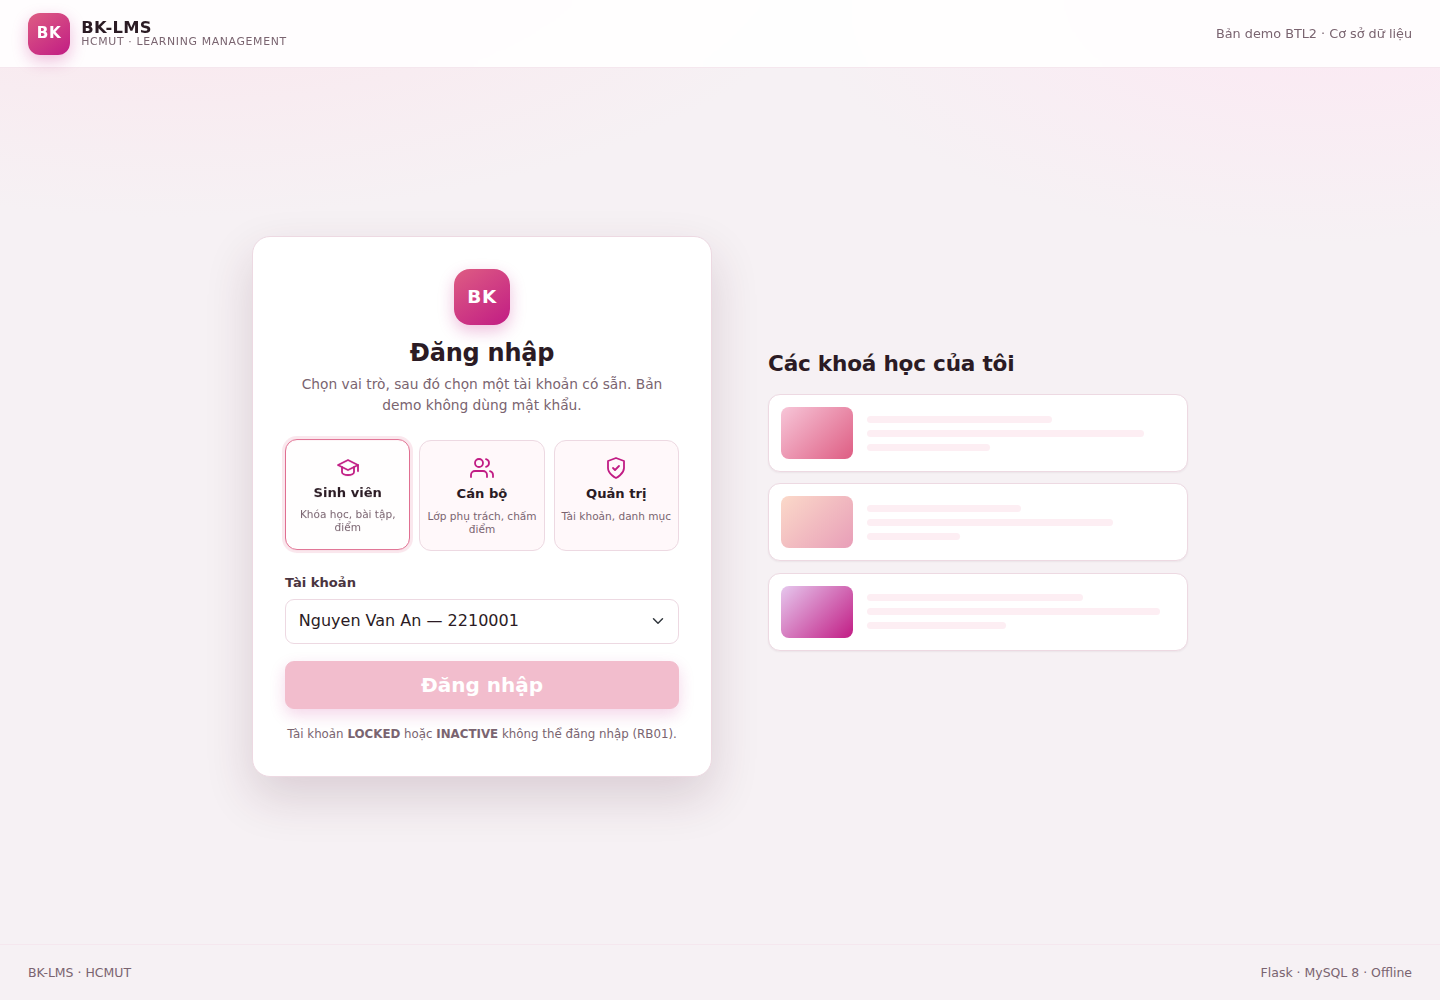
\includegraphics[width=0.92\textwidth]{../docs/evidence/00-login-student.png}
\caption{Màn hình chọn vai trò và tài khoản demo}
\label{fig:login}
\end{figure}

\begin{figure}[H]
\centering
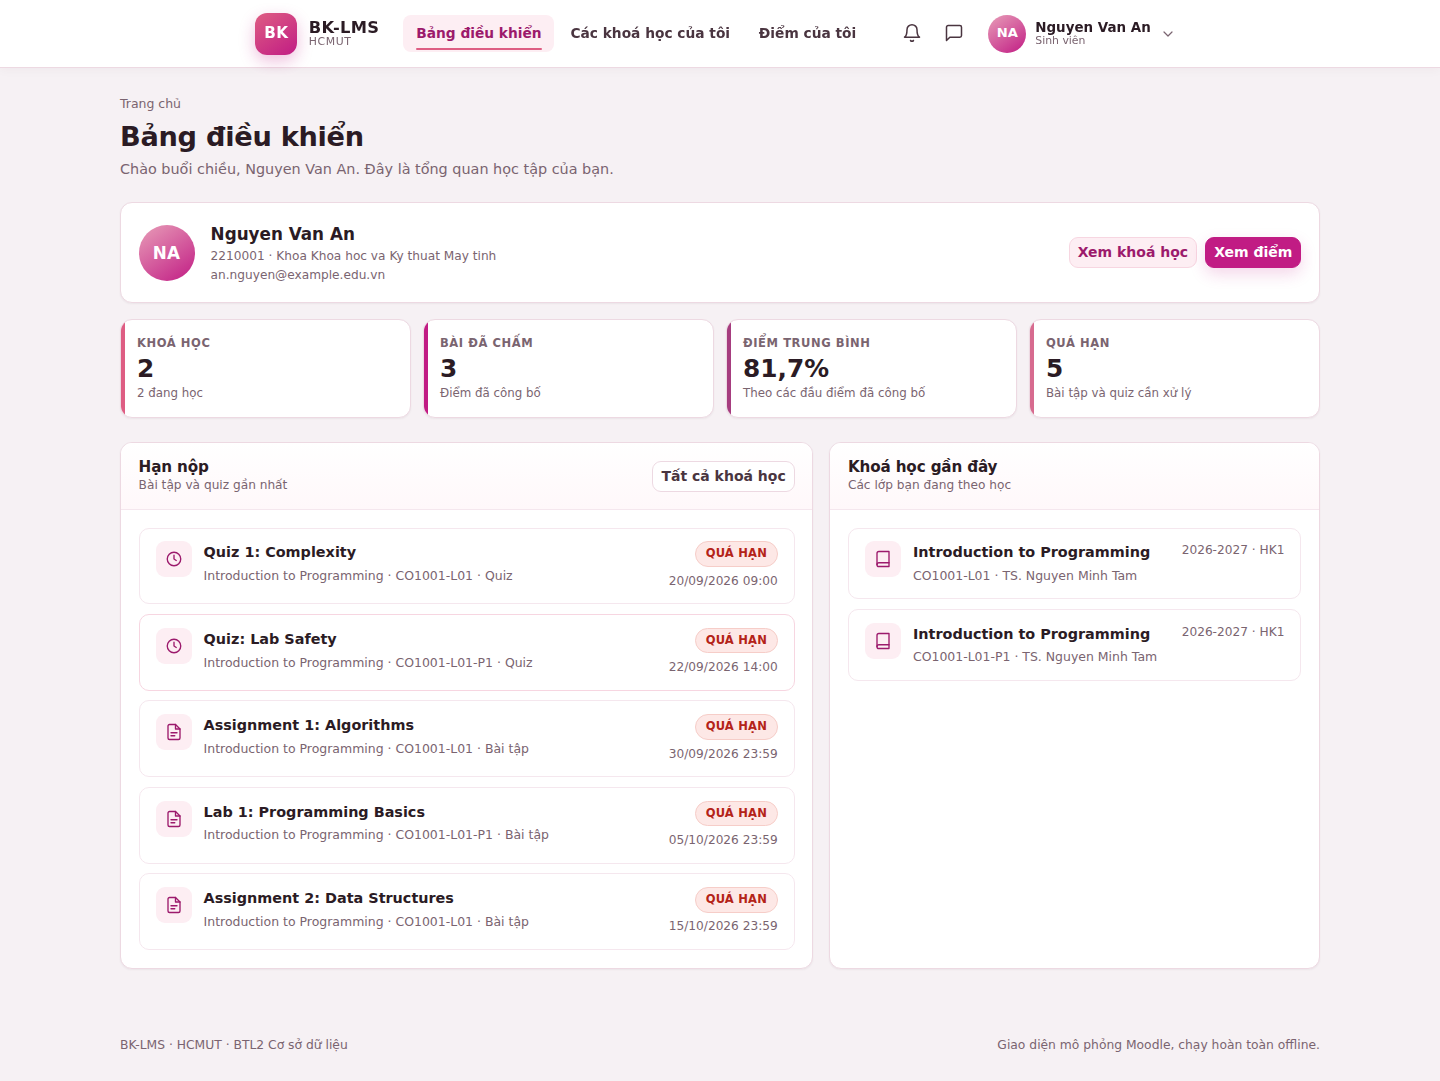
\includegraphics[width=0.92\textwidth]{../docs/evidence/01-student-dashboard.png}
\caption{Dashboard sinh viên}
\label{fig:student-dashboard}
\end{figure}

\begin{figure}[H]
\centering
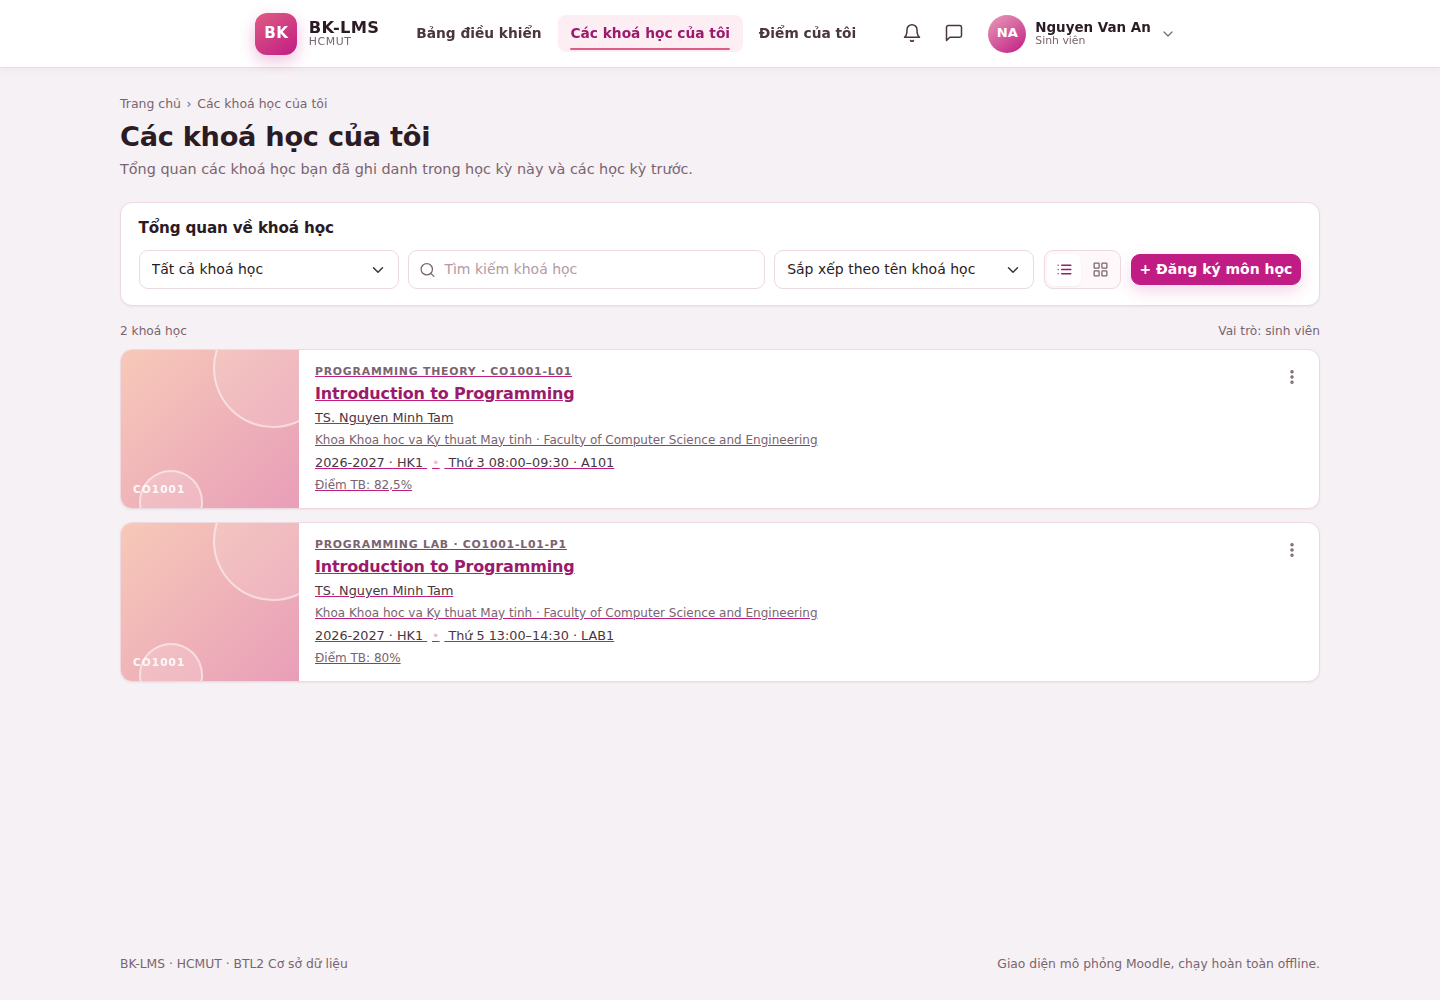
\includegraphics[width=0.92\textwidth]{../docs/evidence/02-student-courses.png}
\caption{Danh sách lớp học phần của sinh viên}
\label{fig:student-courses}
\end{figure}

\begin{figure}[H]
\centering
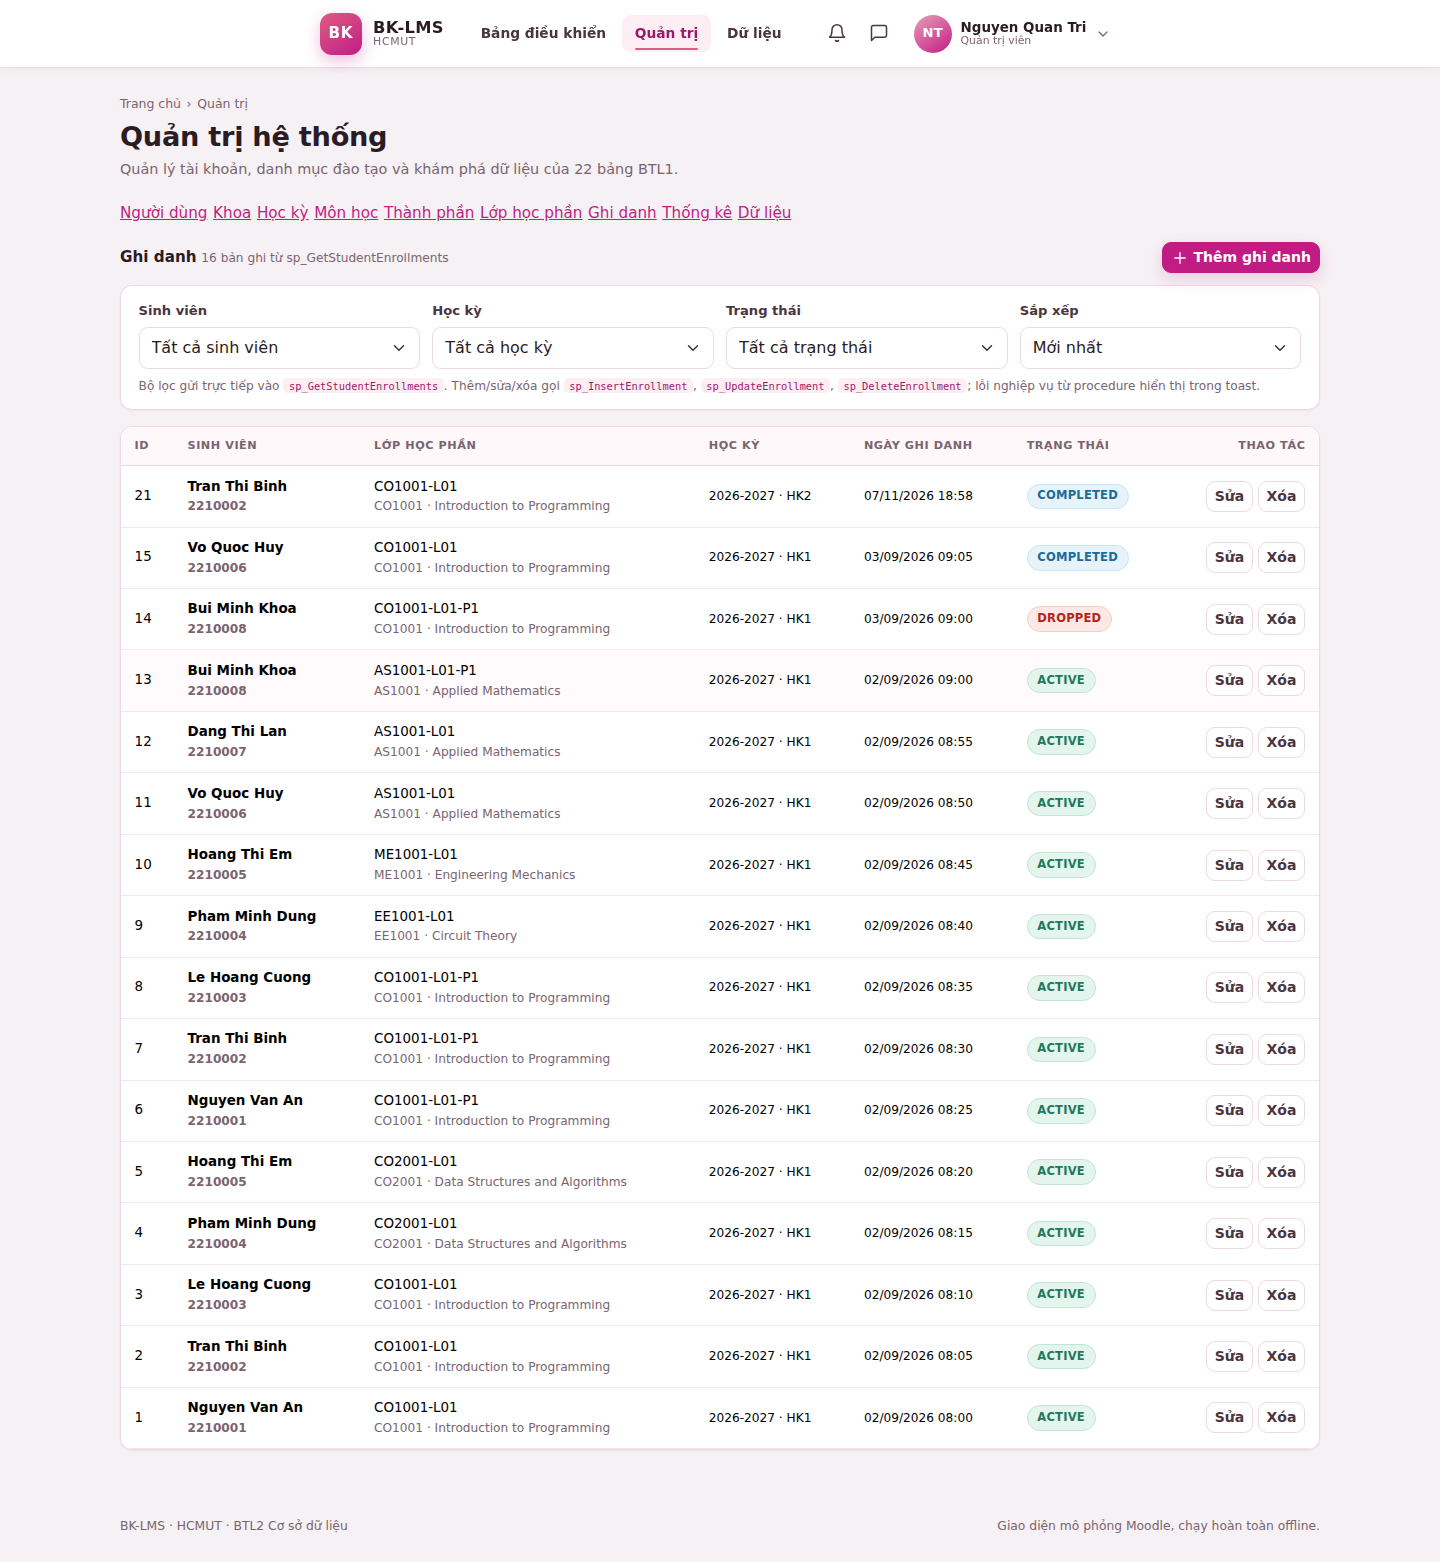
\includegraphics[width=0.92\textwidth]{../docs/evidence/12-admin-enrollments.png}
\caption{Tab Quản trị $\rightarrow$ Ghi danh với bộ lọc và CRUD}
\label{fig:admin-enrollments}
\end{figure}

\begin{figure}[H]
\centering
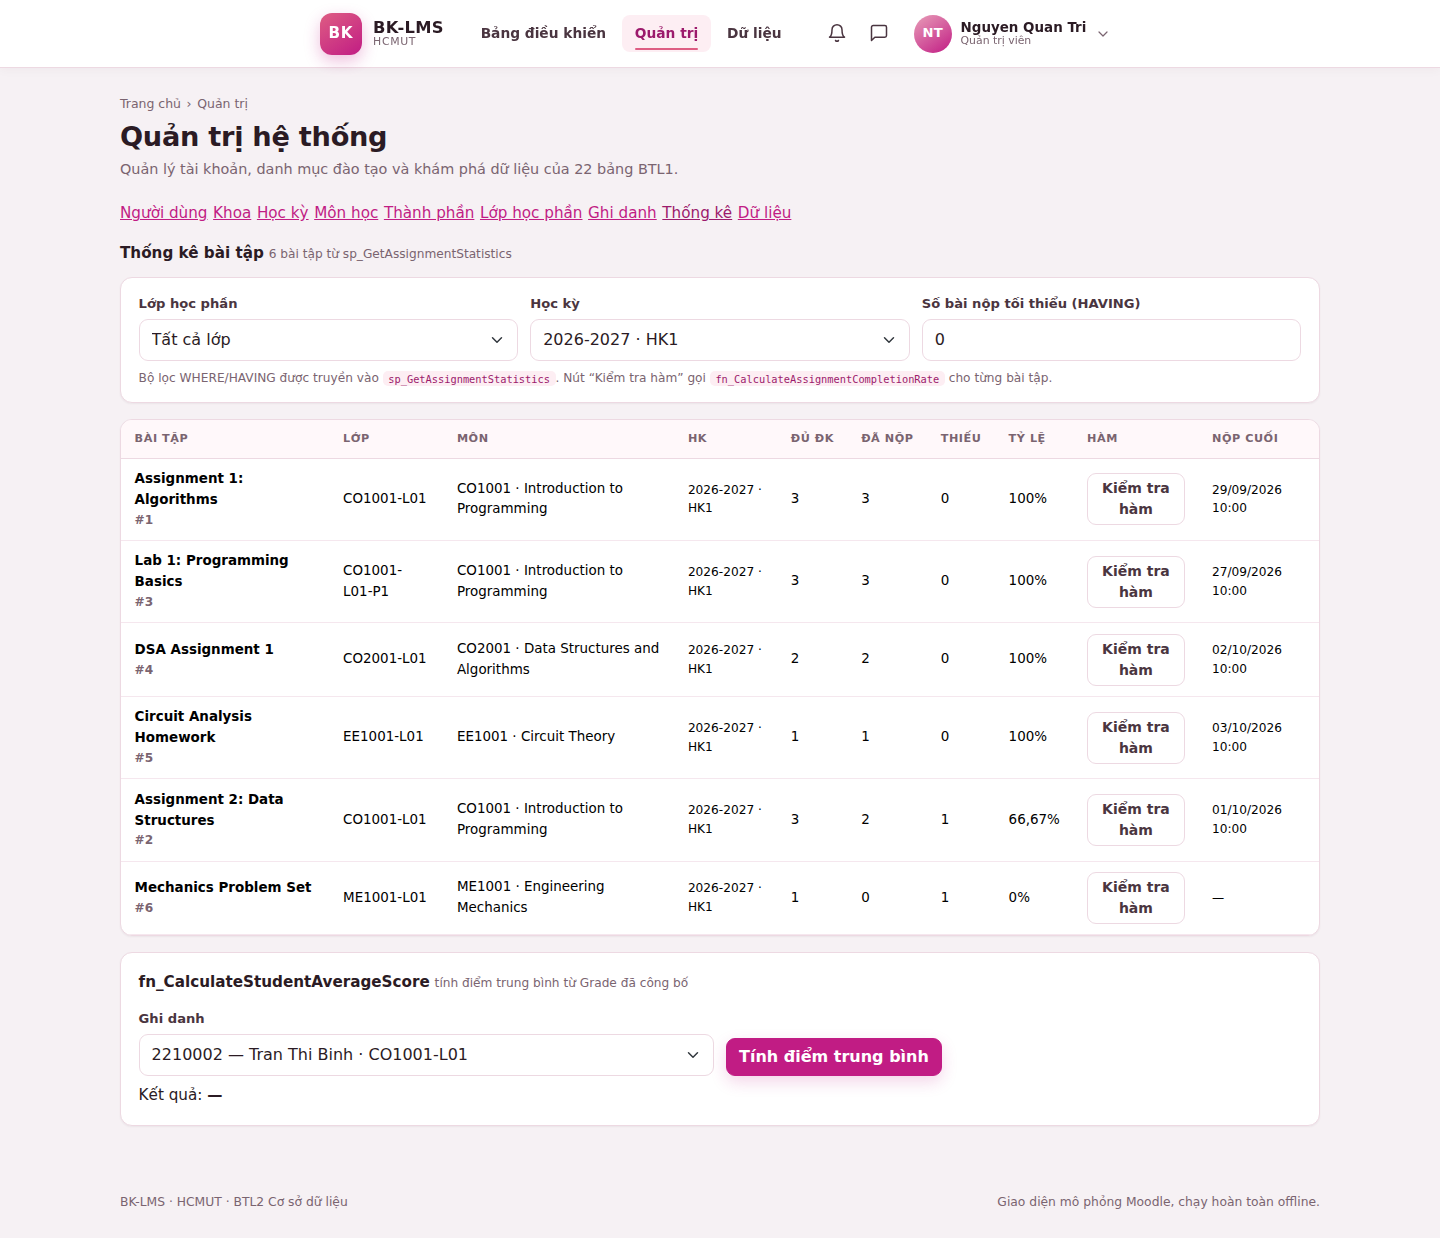
\includegraphics[width=0.92\textwidth]{../docs/evidence/14-admin-statistics.png}
\caption{Tab Quản trị $\rightarrow$ Thống kê gọi procedure và function}
\label{fig:admin-statistics}
\end{figure}

\subsection{Luồng CRUD Ghi danh}

Bảng~\ref{tab:crud-ui} tóm tắt đường đi của từng thao tác. Danh sách lấy dữ liệu từ
\Tbl{sp_GetStudentEnrollments}; thêm/sửa/xóa gọi đúng ba procedure CRUD. Lỗi nghiệp
vụ từ procedure được hiển thị bằng toast đỏ, không làm mất dữ liệu đang nhập.

\begin{table}[H]
\centering
\caption{Luồng UI -- API -- procedure của CRUD Ghi danh}
\label{tab:crud-ui}
{\footnotesize\setlength{\tabcolsep}{3pt}\begin{tabular}{@{}L{2.6cm}L{4.0cm}L{4.0cm}L{4.2cm}@{}}
\toprule
\rowcolor{tableheader}
\textbf{Thao tác} & \textbf{HTTP} & \textbf{Service/Repository} & \textbf{Procedure} \\
\midrule
Danh sách & \Tbl{GET /api/enrollments} & \Tbl{list} & \Tbl{sp_GetStudentEnrollments} \\
Thêm & \Tbl{POST /api/enrollments} & \Tbl{create} & \Tbl{sp_InsertEnrollment} \\
Sửa & \Tbl{PUT /api/enrollments/<id>} & \Tbl{update} & \Tbl{sp_UpdateEnrollment} \\
Xóa & \Tbl{DELETE /api/enrollments/<id>} & \Tbl{delete} & \Tbl{sp_DeleteEnrollment} \\
\bottomrule
\end{tabular}}
\end{table}

\subsection{Cấu hình và chạy}

Ứng dụng chạy bằng \Tbl{uv} và Python 3.12; CSDL chạy bằng Docker MySQL 8.4. Các lệnh
chính:

\begin{lstlisting}[style=sqlstyle,language=bash,caption={Lệnh chạy ứng dụng và kiểm thử},label={lst:run}]
cd hcmut-lms-btl2
uv sync
cp .env.example .env
docker compose up -d mysql
.venv/bin/python scripts/init_database.py
.venv/bin/python run.py
# terminal khac
uv run pytest -q
.venv/bin/python scripts/verify_database.py
.venv/bin/python scripts/smoke_api.py
\end{lstlisting}

% =====================================================================
\section{Kiểm thử}
% =====================================================================

\subsection{Chiến lược kiểm thử}

\begin{table}[H]
\centering
\caption{Các tầng kiểm thử và phạm vi}
\label{tab:test-layers}
\begin{tabular}{@{}L{3.6cm}L{6.4cm}L{4.4cm}@{}}
\toprule
\rowcolor{tableheader}
\textbf{Tầng} & \textbf{Nội dung} & \textbf{Kết quả} \\
\midrule
CSDL & 22 bảng, 13 trigger, 5 procedure, 2 function, seed, ràng buộc & PASS \\
SQL test & 13 file test dương/âm, expected fail & PASS \\
Python & API, service, repository, validation, auth, frontend static & 72 passed \\
Smoke API & Flask + MySQL thật, 3 vai trò, CRUD, 401/403 & 31/31 PASS \\
Browser E2E & Chromium headless: Student, Staff, Admin, CRUD Ghi danh & PASS, không lỗi console \\
\bottomrule
\end{tabular}
\end{table}

\subsection{Kiểm thử CSDL}

Script \Tbl{scripts/verify_database.py} kiểm tra số bảng, trigger, procedure, function,
tính nhất quán của \Tbl{SubmissionCount}, xung đột lịch, kết quả hai function và số
hàng seed tối thiểu. Kết quả thật:

\begin{lstlisting}[style=sqlstyle,language=bash,caption={Kết quả kiểm tra CSDL},label={lst:verify}]
[PASS] table_count = 22
[PASS] trigger_count = 13
[PASS] procedure_count = 5
[PASS] function_count = 2
[PASS] submission_count_mismatches = 0
[PASS] schedule_conflicts = 0
[PASS] completion_rate_assignment_1 = 100.00
[PASS] completion_rate_assignment_6 = 0.00
[PASS] average_score_enrollment_1 = 82.50
[PASS] every one of the 22 tables has at least 5 seed rows
DATABASE VERIFICATION: PASS
\end{lstlisting}

\subsection{Kiểm thử Python}

\begin{table}[H]
\centering
\caption{Các nhóm test Python}
\label{tab:pytest-files}
\begin{tabular}{@{}L{6.4cm}L{7.6cm}@{}}
\toprule
\rowcolor{tableheader}
\textbf{File} & \textbf{Nội dung} \\
\midrule
\Tbl{test_auth.py} & login/logout, role guard, profile, catalog, enroll/drop, quiz, file, không PII \\
\Tbl{test_config.py} & fail-fast SECRET\_KEY ở production \\
\Tbl{test_enrollments_api.py} & CRUD, validation, lỗi procedure, 401/403/200 \\
\Tbl{test_statistics_api.py} & thống kê, function, 401/403/200 \\
\Tbl{test_catalog_api.py} & catalog, bảo vệ \Tbl{/api/students} \\
\Tbl{test_repositories.py} & xác nhận gọi đúng \Tbl{sp_*} / \Tbl{fn_*} \\
\Tbl{test_health.py}, \Tbl{test_validation.py} & health, validation \\
\Tbl{test_json_provider.py}, \Tbl{test_frontend.py} & JSON provider, frontend static \\
\bottomrule
\end{tabular}
\end{table}

Kết quả: \textbf{72 passed}. Các test 401/403 chứng minh API không chỉ ẩn UI mà thực
sự chặn truy cập trực tiếp.

\subsection{Smoke API và phân quyền}

Smoke chạy trên Flask + MySQL thật, gồm 31 check. Bảng~\ref{tab:auth-checks} là các
kiểm tra phân quyền trọng tâm.

\begin{table}[H]
\centering
\caption{Kiểm tra 401/403/200 trên API quản trị}
\label{tab:auth-checks}
\begin{tabular}{@{}L{7.0cm}C{2.2cm}C{2.2cm}C{2.2cm}@{}}
\toprule
\rowcolor{tableheader}
\textbf{Request} & \textbf{Không login} & \textbf{Student} & \textbf{Admin} \\
\midrule
\Tbl{GET /api/enrollments} & 401 & 403 & 200 \\
\Tbl{POST /api/enrollments} & 401 & 403 & 201 \\
\Tbl{GET /api/statistics/overview} & 401 & 403 & 200 \\
\Tbl{GET /api/students} & 401 & 403 & 200 \\
\bottomrule
\end{tabular}
\end{table}

\subsection{Kiểm thử trình duyệt}

Playwright Chromium headless đã chạy các luồng: đăng nhập ba vai trò; Student xem
dashboard, courses, course tabs, assignment, quiz, grades, profile; Staff xem
dashboard, submissions, chấm điểm; Admin xem users/sections, CRUD Ghi danh, Thống kê +
hai function, data explorer. Kết quả không có \Tbl{pageerror} hay lỗi console; ảnh
được lưu trong \Tbl{docs/evidence/}. Chuỗi CRUD thực tế: bảng có 16 dòng, lọc student
101 còn 2 dòng, thêm một dòng, sửa sang \Tbl{DROPPED}, xóa và trở về 16 dòng.

\subsection{Readiness và việc còn lại}

Script \Tbl{scripts/check_submission_readiness.py} kiểm tra tài liệu, số test, cấu
trúc source và các artefact bắt buộc. Kết quả hiện tại chỉ còn FAIL vì
\Tbl{docs/TEAM_ASSIGNMENT.md} chưa điền tên/MSSV. Đây là P0 của con người, không phải
lỗi code.

% =====================================================================
\clearpage
\section{Phân công, kết luận và hạn chế}
% =====================================================================

\subsection{Phân công thành viên}

{\footnotesize\setlength{\tabcolsep}{3pt}\begin{longtable}{@{}L{1.1cm}L{3.1cm}L{4.1cm}L{6.2cm}@{}}
\caption{Phân công 5 thành viên và object sở hữu}
\label{tab:team}\\
\toprule
\rowcolor{tableheader}
\textbf{TV} & \textbf{Họ tên -- MSSV} & \textbf{Vai trò} & \textbf{SQL object / phần phụ trách} \\
\midrule
\endfirsthead
\toprule
\rowcolor{tableheader}
\textbf{TV} & \textbf{Họ tên -- MSSV} & \textbf{Vai trò} & \textbf{SQL object / phần phụ trách} \\
\midrule
\endhead
\bottomrule
\endfoot
TV1 & [Họ tên] -- [MSSV] & Database lead & \Tbl{trg_section_schedule_bi/bu}, \Tbl{trg_feedback_validate_bi/bu} \\
TV2 & [Họ tên] -- [MSSV] & CRUD \& backend & \Tbl{sp_Insert/Update/DeleteEnrollment}, API/UI Ghi danh \\
TV3 & [Họ tên] -- [MSSV] & Integrity \& seed & \Tbl{trg_enrollment_capacity_bi/bu}, \Tbl{trg_grade_validate_bi/bu} \\
TV4 & [Họ tên] -- [MSSV] & Query \& function & 2 query procedure, 2 function, tab Thống kê \\
TV5 & [Họ tên] -- [MSSV] & Submission \& UI/ops & 5 trigger submission, frontend, script Windows \\
\end{longtable}}

Mỗi thành viên phải điền tên/MSSV, commit gắn với object mình sở hữu và chạy
\Tbl{git shortlog -sne --all} để đối chiếu. Bảng đầy đủ và câu hỏi demo nằm trong
\Tbl{docs/TEAM_ASSIGNMENT.md} và \Tbl{docs/DEMO_SCRIPT.md}.

\subsection{Kết luận}

Bài tập đã hiện thực đầy đủ mô hình BTL1 thành 22 bảng quan hệ với 35 khóa ngoại,
10 UNIQUE, 39 CHECK và 15 index. Các quy tắc liên bảng được cài đặt bằng 13 trigger;
nghiệp vụ ghi danh được đóng gói trong 3 procedure CRUD có transaction; hai procedure
truy vấn đáp ứng JOIN/WHERE/ORDER BY/aggregate/GROUP BY/HAVING; hai function có
cursor/IF/LOOP và được gọi thật từ giao diện. Ứng dụng Flask + SPA phân quyền ba vai
trò, gọi procedure/function thật, và đã được kiểm thử ở mức CSDL, API và trình duyệt.

\subsection{Hạn chế và hướng phát triển}

\begin{table}[H]
\centering
\caption{Hạn chế đã biết và hướng khắc phục}
\label{tab:limitations}
\begin{tabular}{@{}L{6.0cm}L{8.0cm}@{}}
\toprule
\rowcolor{tableheader}
\textbf{Hạn chế} & \textbf{Hướng khắc phục} \\
\midrule
Không có xác thực bằng mật khẩu; chỉ chọn tài khoản demo & Tích hợp CAS/OAuth hoặc password hash + session thật \\
Chưa có CSRF token & Thêm CSRF token cho form/POST hoặc dùng SameSite + token \\
Chưa kiểm thử Windows thật & Chạy \Tbl{setup.bat} trên máy Windows sạch, ghi log \\
Chưa kiểm thử Firefox/Safari/Edge & Bổ sung Playwright đa trình duyệt \\
Chưa kiểm thử tải/đồng thời quy mô lớn & Dùng Locust/k6, đo khóa \Tbl{FOR UPDATE} và deadlock \\
RB04/RB06 chưa ép đầy đủ bằng trigger & Bổ sung kiểm tra nhóm lý thuyết--thực hành ở procedure/service \\
Tệp đính kèm chỉ lưu metadata & Bổ sung storage thật, kiểm tra MIME/size, virus scan \\
\bottomrule
\end{tabular}
\end{table}

% =====================================================================
% APPENDICES
% =====================================================================
\clearpage
\appendix
\section{Mã schema tiêu biểu}
\label{app:schema}

Toàn bộ DDL nằm trong \Tbl{database/schema/01_tables.sql}. Dưới đây là phần đầu của
file, gồm các bảng định danh và học vụ.

\lstinputlisting[style=sqlappendix,firstline=1,lastline=100,
    caption={Trích \Tbl{01_tables.sql}: bảng định danh và học vụ},
    label={lst:schema-excerpt}]{../database/schema/01_tables.sql}

\section{Mã trigger tiêu biểu}
\label{app:triggers}

\lstinputlisting[style=sqlappendix,firstline=11,lastline=45,
    caption={Trigger \Tbl{trg_section_schedule_bi}},
    label={lst:trg-schedule}]{../database/triggers/05_triggers.sql}

\lstinputlisting[style=sqlappendix,firstline=116,lastline=140,
    caption={Trigger \Tbl{trg_submission_count_au}},
    label={lst:trg-count}]{../database/triggers/05_triggers.sql}

\section{Mã procedure tiêu biểu}
\label{app:procedures}

\lstinputlisting[style=sqlappendix,firstline=16,lastline=60,
    caption={\Tbl{sp_InsertEnrollment}: phần đầu và validation},
    label={lst:proc-insert-1}]{../database/procedures/06_procedures.sql}

\lstinputlisting[style=sqlappendix,firstline=61,lastline=110,
    caption={\Tbl{sp_InsertEnrollment}: transaction và insert},
    label={lst:proc-insert-2}]{../database/procedures/06_procedures.sql}

\section{Mã function}
\label{app:functions}

\lstinputlisting[style=sqlappendix,firstline=1,lastline=80,
    caption={\Tbl{fn_CalculateAssignmentCompletionRate}},
    label={lst:fn-completion}]{../database/functions/07_functions.sql}

\lstinputlisting[style=sqlappendix,firstline=81,lastline=145,
    caption={\Tbl{fn_CalculateStudentAverageScore}},
    label={lst:fn-average}]{../database/functions/07_functions.sql}

\section{Lệnh kiểm tra và checklist nộp bài}
\label{app:checklist}

\begin{lstlisting}[style=sqlstyle,language=bash,caption={Chạy lại toàn bộ kiểm thử},label={lst:final-check}]
cd hcmut-lms-btl2
uv run pytest -q                         # 72 passed
.venv/bin/python scripts/verify_database.py
.venv/bin/python scripts/smoke_api.py    # Flask phai dang chay
.venv/bin/python scripts/check_submission_readiness.py --with-tests
\end{lstlisting}

Checklist trước khi nộp:

\begin{enumerate}
    \item Điền họ tên/MSSV vào bảng phân công và trang bìa.
    \item Mỗi thành viên có commit gắn với SQL object mình sở hữu.
    \item Chạy lại 4 lệnh trên máy sạch; lưu log.
    \item Chạy \Tbl{check_environment.bat} trên Windows thật nếu có.
    \item Kiểm tra \Tbl{.env} không bị commit.
    \item Đính kèm PDF báo cáo và ảnh minh chứng nếu giảng viên yêu cầu.
\end{enumerate}

\end{document}
